\documentclass[12pt, a4paper]{memoir} % for a short document
\usepackage[french,english]{babel}

\usepackage [vscale=0.76,includehead]{geometry}                % See geometry.pdf to learn the layout options. There are lots.
%\geometry{a4paper}                   % ... or a4paper or a5paper or ... 
%\geometry{landscape}                % Activate for for rotated page geometry
%\OnehalfSpacing
% \setSingleSpace{1.05}
%\usepackage[parfill]{parskip}    % Activate to begin paragraphs with an empty line rather than an indent


%===================================== packages
\usepackage{lipsum}
\usepackage{graphicx}
\usepackage{amsmath}
\usepackage{fullpage}
\usepackage{mathptmx} % font = times
\usepackage{helvet} % font sf = helvetica
\usepackage[latin1]{inputenc}
\usepackage{relsize}
\usepackage[T1]{fontenc}
\usepackage{tikz}
\usepackage{booktabs}
\usepackage{textcomp}%textquotesingle
\usepackage{multirow}
\usepackage{pgfplots}
\usepackage{url}
\usepackage{footnote}
\usepackage[style=numeric,sorting=none]{biblatex}
\bibliography{bibfile.bib}
\usepackage{hyperref}
\setlength\beforechapskip{-\topskip} %% remove blank above chapter title
\usepackage{color}
\usepackage{hyperref}
\hypersetup{colorlinks,
    linkcolor = black,
    %citecolor=blue
}
\usepackage{graphicx}
\usepackage{amsmath,amsfonts,amssymb}

%============================================
\usetikzlibrary{arrows,shapes,positioning,shadows,trees}
\makesavenoteenv{tabular}
\makesavenoteenv{table}
%==============================================
\def\checkmark{\tikz\fill[scale=0.4](0,.35) -- (.25,0) -- (1,.7) -- (.25,.15) -- cycle;}
%Style des têtes de section, headings, chapitre
\headstyles{komalike}
\nouppercaseheads
\chapterstyle{dash}
\makeevenhead{headings}{\sffamily\thepage}{}{\sffamily\leftmark} 
\makeoddhead{headings}{\sffamily\rightmark}{}{\sffamily\thepage}
\makeoddfoot{plain}{}{}{} % Pages chapitre. 
\makeheadrule{headings}{\textwidth}{\normalrulethickness}
%\renewcommand{\leftmark}{\thechapter ---}
\renewcommand{\chaptername}{\relax}
\renewcommand{\chaptitlefont}{ \sffamily\bfseries \LARGE}
\renewcommand{\chapnumfont}{ \sffamily\bfseries \LARGE}
\setsecnumdepth{subsubsection}


% Title page formatting -- do not change!
\pretitle{\HUGE\sffamily \bfseries\begin{center}}
\posttitle{\end{center}}
\preauthor{\LARGE  \sffamily \bfseries\begin{center}}
\postauthor{\par\end{center}}
\newcommand{\jury}[1]{% 
\gdef\juryB{#1}} 
\newcommand{\juryB}{} 
\newcommand{\session}[1]{% 
\gdef\sessionB{#1}} 
\newcommand{\sessionB}{} 
\newcommand{\option}[1]{% 
\gdef\optionB{#1}} 
\newcommand{\optionB} {}

\renewcommand{\maketitlehookd}{% 
\vfill{}  \large\par\noindent  
\begin{center}\juryB \bigskip\sessionB\end{center}
\vspace{-1.5cm}}
\renewcommand{\maketitlehooka}{% 
\vspace{-1.5cm}\noindent
\includegraphics[height=12ex]{pics/logo-uga.png}\hfill\raisebox{2ex}{
\includegraphics[height=14ex]{pics/logoINP.png}}\\
\bigskip
\begin{center} \large
Master of Science in Informatics at Grenoble \\
Master Informatique \\ 
Specialization \optionB  \end{center}\vfill}
% =======================End of title page formatting
\title{Deep learning for visual attention in chess}
\option{Graphics, Vision, Robotics} 
\small {\author{Justin Le Louedec}}
\date{Juin, 2018} % Delete this line to display the current date
\jury{
Research project performed at YOUR LAB \\\medskip
Under the supervision of:\\
Your Supervisor\\\medskip
Defended before a jury composed of:\\
Head of the jury\\
Jury member 1\\
Jury member 2\\
}
\session{Month \hfill 2017}
\setcounter{tocdepth}{4}
\setcounter{secnumdepth}{4}

%%% BEGIN DOCUMENT
\begin{document}
\selectlanguage{English} % french si rapport en français
\frontmatter
\begin{titlingpage}
\maketitle
\end{titlingpage}

%\small
\setlength{\parskip}{-1pt plus 1pt}

\renewcommand{\abstracttextfont}{\normalfont}
\abstractintoc
\begin{abstract} 
Your abstract goes here... 
\end{abstract}
\abstractintoc

\renewcommand\abstractname{Acknowledgement}
\begin{abstract}
I would like to express my sincere gratitude to .. for his invaluable assistance and comments in reviewing this report... 
Good luck :) 
\end{abstract}


\renewcommand\abstractname{R\'esum\'e}
\begin{abstract} \selectlanguage{French}
Your abstract in French goes here... 
\end{abstract}
\selectlanguage{English}

\cleardoublepage

\tableofcontents* % the asterisk means that the table of contents itself isn't put into the ToC
\normalsize

\mainmatter
\SingleSpace
%==============================CHAPTERS==================
\chapter{Introduction}
%\lipsum[2-4]

\section{Visual attention modeling, deep learning and chess expertise}

Our work is part of the Ceege project \footnote{\url{https://ceege.inria.fr/}}, a multidisciplinary research project, which aim to produce a mental model of chess players to predict their expertise. We present in this report our work on modeling visual attention of chess players for problem solving tasks.

One of the particularity of Humans is there incredible ability to discriminate and select information from their surrounding world instead of processing entire scenes all at once. This selective attention is  really important and allows us to quickly interpret and understand our environment to interact with it. The simulation of this process is commonly referred as visual attention prediction or visual saliency detection. It is a very active research topic in computer vision and neuroscience. Modelling visual attention not only allows us to understand a bit more how human visual system works but it has also a lot of applications. Among them we have object recognition/detection \cite{saliencydetection,saliencydetectionvideo,Buso2015}, action recognition \cite{DBLP:journals/corr/SafaeiF17,phdthesis}, object segmentation \cite{10.1007/978-3-319-01796-9_31,7984578}, or  even applications in computer graphics \cite{3Dshapevisualattention,phdthesis2}.\\ 

The sub-branch of machine learning, called Deep learning consists of multiple layer of neurons applying non linear function on large amount of data to extract features from it and learn them. These deep learning algorithms have seen their popularity increase for the past 10 years due to more powerful graphical processing units (GPUs) and larger quantity of data \cite{imagenet_cvpr09} and more powerful algorithms \cite{NIPS2012_4824}. But the general idea behind deep learning was already there from the 1990s, but their importance decrease with support vector machines (SVMs). Convolutional neural networks (CNNs) are multistage architecture composed of non-linear layer and primarily convolution, extracting features from large dataset, to classify it, do detection/segmentation tasks  or coupled with other methods such as Natural language processing (NLP), or reinforcement learning (RL) can be used for other task such as playing games \cite{DBLP:journals/corr/MnihKSGAWR13}, controlling robots \cite{DBLP:journals/corr/Amarjyoti17}, and translating languages into others   \cite{DBLP:journals/corr/ChoMGBSB14}or semantic segmentation \cite{shen2014learning}. More about them can be found in Annexe \ref{Annexe:deeplearning}.\\

chess expertise

Modeling visual attention for chess players has several benefits. Being able to predict where chess players depending on their level would look at, would allow us for a given player to assess his level depending on where he looks. This could also be a way to help players, by highlighting relations and pattern between pieces that are relevant. Or even challenging players by blurring the part of the board they would look at.





\section{Premises and requirements}

The problem behind this project is to create a model able to create a prediction of chess players attention. The model, given a picture of a chessboard in a specific configuration, should be able to produce a salient map illustrating region that would be attended by a chess player. The model should be based on a deep learning approach, trained on eye-gazing data captured from chess players doing problem solving tasks.

In this report we are going to appraise if it is possible to model visual attention of chess players using deep learning techniques and eye-gazing heatmaps from chess players. We will also see if it is possible to use our data as they are and what processing should be done. Finally we investigate the creation of a new dataset to help the modelling of visual attention for chess problem solving task.




\section{}
 
Approx  1 to 2  page description of the scientific approach or approaches to a solution and how it was   investigated and evaluated.  Present a summary of the principal results obtained

\section{}
Summarize the contents of the subsections of each chapter. Give the topics addressed and summarize what is written in each chapter. 

\chapter{Background and related work} \label{SoA}

This Chapter is meant to introduce Visual attention and how it can be modelled and evaluated.\\
Firstly we give an introduction and overview of visual attention modeling in section \ref{Introduction to Visual Attention}. Finally we will discuss Chess visual expertise in section \ref{Chess expertise and eye tracking}.
%%and finally we will introduce important layers used in our Deep learning model (section \ref{Deep learning}).

\section{ Introduction to Visual Attention} \label{Introduction to Visual Attention}

Visual attention is a biological system allowing living creature to select interesting and relevant regions from a visual scene. This gives the opportunity to higher-level cognitive functions to execute more complex task such as scene understanding or decision making while not having to focus on too much data. In cognitive neuroscience visual attention is referred as a neural system selecting information from the visual system. In his paper Posner \cite{posner1990} formulate the idea that visual attention is not the function of a singular area of the brain but rather the result of a network of different parts. He also explains that pattern recognition  is about how successions of neurons process visual stimulus to detect such information. 

Visual attention can be categorized in two ways :
\begin{itemize}
    \item Bottom-up approach : information is taken from the scene based on objects and part of the scene saliency.
    \item Top-Down : Attention is driven by task or action to accomplished based on a prior knowledge and/or the action the observer seeks to accomplish.
\end{itemize}
These two approaches are related to the two main visual attention methods. The first one being the exogenous, which is how attention component are determined by external stimulus characteristics (ie. bright object, high contrast between a hand and a background, straight lines etc..) . The second one is the endogenous, is determined by the user intentions and actions (ie. moving a chess piece, grabbing something).\\ Attention can also be described as overt or covert. Overt happens when the subject is moving his gazing point from one point to the other in the scene. Covert attention on the other hand  is also a shift in the attention/gazing point to a new location in the attention scene, but using the fovea and not a  motor action (ie. Sharp vision at a point of the scene).

Eye tracking systems detect where human eyes are fixating and they path their eyes follow. These fixations are also characterized by the time spent on different parts of the scene. These graphs of fixations and path can be used as indicators on most viewed and fixated areas on images or scenes. They are often transformed to continuous saliency maps by convoluting Gaussian functions with an higher intensity depending on the duration of fixation. Figure \ref{fig:exampleeye} shows an example of eye tracking data with in the background a chess configuration. The points are fixations with their value inside them depending on the time the user fixated this area. The line between two point is the path the eye followed between two fixations. This data was acquired through experimentation for the paper of Thomas Guntz \cite{thomasguntz}. He worked on observing and interpreting subjects in problem solving task (chess in particular) through multimodal observation (Eye tracking, posture, emotion etc...).

\begin{figure}
    \centering
    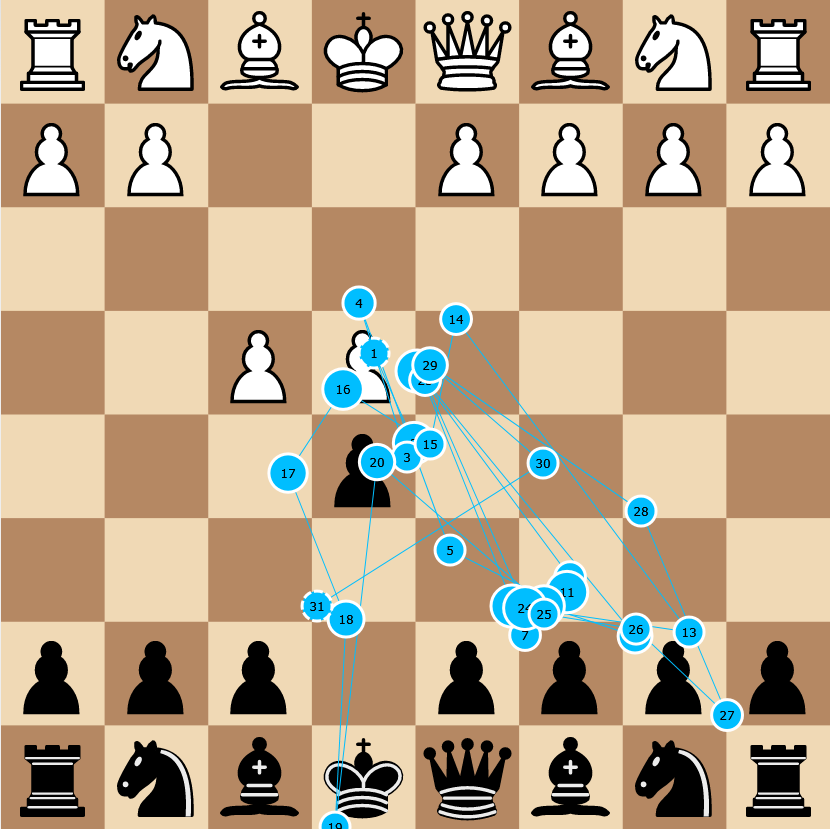
\includegraphics[scale=0.35]{./dataset/image.png}
    \caption{An example of eye tracking data for an user on a chess configuration}
    \label{fig:exampleeye}
\end{figure}

Eye tracking maps captured on human looking at a simple scene with one or few salient objects, show that they tend to notice only the main objects and ignore the background.
Chess and other board game  are particular cases for visual attention, as salient object are essentially the pieces, but their saliency is determined by their move and the current configuration of the game.



\subsection{Visual attention modeling}

Visual attention has already been subject to modeling in 1995 before the impressive development of Deep neural network , in the artificial intelligence book by Tsotsos and al \cite{tsotsos1995}.  They used a pyramidal system composed of layers and filter applied to features maps and producing saliency maps. Their work is very close to what we see nowadays with neural network and produced simple but encouraging results proving that visual attention could be modeled. Their model is based on the idea of selective tuning, features are taken from the scene and used to decide which part of it should be the center of attention, using a hierarchy of a new WAT (winner takes all) algorithm. in overall their model is strongly inspired by primate biological visual attention system, and links to biological processes such as foveating and eye movement are investigated.  \\


In their paper, Borji and Itti \cite{Borji} offer a review of techniques used in Visual attention modeling until 2013. Giving a clear overview of  different model categories such as Bayesian models, cognitive models, graphical models or spectral analysis models. Metrics are also discussed and giving a comparison between performances and approaches, they forecast what the future of visual attention modeling could be.
Circa 2012, the Deep learning field\cite{krizhevsky2012imagenet,szegedy2015going,DBLP:journals/corr/MnihKSGAWR13,jia2014caffe,5537907,deng2009imagenet,srivastava2014dropout} became the center of attention on the visual attention scene, mainly because it is a very good way to extract features automatically and use them in a bottom-up approach.
In their paper Ba and al. \cite{BaMK14}, proposed a Recurrent network model, based on visual attention to improve state of the art performances in multiple number recognition and localization. This work shows the importance of having a focused attention when comes the need to recognize an object or to locate it. However these networks learned attention, was quite different from the human one and as we are trying to model the human attention it was impossible to use the one of those network.
Xu and al. \cite{xu2015show}, worked on using salient part of the images to help a network focus its attention and generate description of images. They proposed a model capable of switching its attention between salient areas and background to offer a description of the image such as "The giraff is standing in the forest", putting in relation objects and their environment.

Visual question answering is very close to visual attention problem as for this task the network focus its attention over a region in a image to answer a question, the same way chess players would do. This is closer to the top-down approach, as the network is given an action to execute based on what he perceive. If we take apart the textual part of the problem, we end up with a "where to look at" and "what is the network looking at" problem. This is what Shih and al. \cite{DBLP:journals/corr/ShihSH15} try to tackle in their paper, where they try to find a way to express the relevancy of a region considering a question.
But most of the time as in the paper from Yang and al. \cite{DBLP:journals/corr/YangHGDS15}, attention is not really the center of preoccupation.\\

In this section we will see several ways to model visual attention before describing other methods based on deep learning (section \ref{subsub:deeplearning}).
\subsubsection{Baseline models}

Before the usage of modern deep learning techniques, a lot of model were proposed showcasing good results and interesting information about human visual attention. Some of them are presented here to give a brief idea about how we came to deep learning.\\


\textbf{Judd Model:  }In their model Judd and al. \cite{judd} worked on predicting human fixations on images. Their work has been focused on gathering data and user eye tracking fixations maps and analyzing the created dataset. Their model is composed of several SVM \cite{Cortes1995} (machine learning classification algorithm), trained on various features group (faces, colors etc..) and combined together in the end to predict fixations. Their work is remarkable for the dataset provided for future research as it was the first dataset with held-out human eye movements and is now often used as a benchmark dataset. It is composed of 300 natural indoor and outdoors scenes with 39 observers.\\


\textbf{Saliency from overt and covert mechanisms:  }In their paper, Itti and Koch \cite{ITTI20001489} proposed a model capable of attend salient locations based on different modalities such as intensity, color, or orientation. By applying filters at various scale they extract feature maps, normalized and centered and then combined to form the final saliency map. Their approach is limited to bottom-up approach but raised some good performances and helped to address how much human we carry information via saliency maps and how it can be tested.\\

\textbf{Task specific Visual Scanpath:  }Mathe and Sminchisescu \cite{NIPS2013_5196}, proposed an important dataset in visual an task driven attention, with over 1 Million fixations in 9157 images. They also developed a Markov model capable of discovering Areas of Interest (AoI), determine from eye tracking data their number, their spatial support, locations, and transition between them. They finally proposed eye movement prediction models based on reinforcement learning and advanced computer vision operators, to learn task specific visual search patterns. \\

\textbf{Bruce Model:  }The model proposed by Bruce and Tsotsos \cite{doi:10.1167/9.3.5}, is based on feature extraction (from vision operators and principal component analysis), and density estimation. Results obtained were showing great efficacy in fixation prediction as compared to other models at that time.

\subsubsection{Deep learning approaches} \label{subsub:deeplearning}
As seen previously, non deep learning models were based on known features such as colors, orientations, gradient, intensity etc.. Deep learning is based on automatic extraction of features from data and then classification, segmentation or other operations. We are going to see few deep learning approaches here, to illustrate different way  how saliency map for visual attention prediction, can be produced.\\

\textbf{SALICON:  }In 2015, SALICON \cite{7410395} was a paper proposing a novel technique based on Deep Neural Networks and object recognition for predicting visual attention. They based their work on the gap of predicting eye fixation with a big semantic content, and previous method proposed, thanks to the high-level encoding in Deep neural networks. They worked on fine-tuning the network with objective functions based on saliency evaluation and by integrating information from the image at different scales. Even today this model is still ranked with the top scores on most of the metrics (described in section \ref{seq:metrics}. 0.87 with AUC-Judd,0.74 linear correlation etc..).

\textbf{Deep fix :  }Deepfix \cite{DBLP:journals/corr/KruthiventiAB15} is a fully convolutional model learning features at different scale, but thanks to a "Location biased convolution layer" it allows to model location dependent patterns. This location problem is addressed by concatenating Gaussian blobs to the input of the convolution layer. They also introduced inception layers to extract complex semantic a different scales level and  to capture global context with large receptive fields.\\

\textbf{Deep Gaze 2:  }DeepGaze 2 \cite{Kummerer_2017_ICCV} is a network meant to be simpler than previous approaches with a pre-trained first part based on VGG19\cite{DBLP:journals/corr/SimonyanZ14a} followed by a readout network. The readout network is a succession of 1*1 convolutions producing a saliency map which is then blurred and transformed into a probability distribution by a softmax function. It uses log likelihood as a loss function to optimize. It produces to this day the best result for the AUC-Judd metric (0.88).\\

\textbf{Salgan: }Finally SalGAN \cite{DBLP:journals/corr/PanCMOTSN17} offers a complete different approach from what we have seen before. This network is a Generative adversarial Networks (GAN \cite{2014arXiv1406.2661G}) composed of a generator and a discriminator. The latter is composed of convolutions (here trained from scratch), follows by  pooling functions  and a fully connected last part. The Generator is an autoencoder , with a first part composed of a VGG network followed by upsampling functions and  a sigmoid. A binary cross entropy loss is computed between the saliency map generated by the generator and the ground truth. Both ground truth and predicted saliency map are given as input to the discriminator which is then  doing predicting and  training using adversarial loss.
This paper is also interesting as it gives a comparative analysis between the Binary cross entropy loss and the Mean square error loss, two loss which can be used with autoencoder, for saliency map generation.

\textbf{Deep visual attention:  } Deep visual attention \cite{DBLP:journals/corr/WangS17b} is a recent paper aiming to leverage multi-scale features for attention prediction model. They use and autoencoder but the decoder is separated into several part, each of them predicting saliency 
for the output of different layers of the encoder. The prediction of the encoders are fused using a last convolutional layer. Their work not only figure in the best performances for attention prediction in view-free scenes (0.85 for AUC-Judd and 0.688 for linear correlation, on the MIT300 dataset \cite{Judd_2012}), but also propose a way to take in consideration multi-scale and spatial relationship in them.


From what we have seen, there exists many ways of approaching visual attention prediction using deep learning. Because of the relations between pieces in chess and the importance of using various scales of features to recognize pieces and moves, we choose to base our model on the Deep visual attention model \cite{DBLP:journals/corr/WangS17b}, but adding some changes as we will see in section \ref{section:model}.

\subsection{Measuring Visual attention}\label{seq:metrics}
To measure quality of saliency map, we consider them as probability distribution. Several metrics can be used and some of them are explained in this section of the report. More about those metrics and some others can be found it Bylinskii and al. \cite{metricsreview}, where they explain the interpretation that can be done depending on the results we can get. They also show how changing the distribution create variation on the results.THree years before Le Meur and Baccinon \cite{LeMeur2013}, proposed a survey for various models for visual attention where they emphasize the use of some methods to benchmark computational models of visual attention.
In this section we will present some of the main metrics used in visual attention prediction.

\subsubsection{Normalized Scanpath Saliency}
Normalized Scanpath Saliency was introduced in Peters and al. paper \cite{Peters2005ComponentsOB}, as a correspondence measure between a normalized saliency map a ground truth at fixations. It is sensible to false positives, relative differences  in  saliency  across  the  image,  and  general   monotonic  transformations. But because of the mean saliency value being subtracted, it is robust to linear transformations. The formula to compute this metric is given in equation \ref{eq:NSS}, Q being our binary ground truth and P the saliency map produced by our model. 

\begin{equation}  
\begin{aligned}
    NSS(P,Q) = \frac{1}{N} \sum\limits_{i=0}^n \bar{P_i} * Q_i\\
    \textrm{where} \quad  \bar{P}= \frac{P - \mu(P)}{\sigma(P)} \quad \textrm{and} \quad  N =  \sum\limits_{i=0}^n Q_i
\end{aligned}
\label{eq:NSS}
\end{equation}
With a value above 0, this metric expresses a correspondence above chance between the two saliency, and below 0 an anti-correspondence.

\subsubsection{Similarity}
Similarity or also referred as histogram intersection is the sum of minimums of two normalized saliency maps. It is defined in equation \ref{eq:SIM} where P is the saliency map produced by the model, and Q the ground-truth.
\begin{equation}  
\begin{aligned}
    NSS(P,Q) = \sum\limits_{i=0}^n min(P_i, Q_i)\\
    \textrm{where} \quad \sum\limits_{i=0}^n P = \sum\limits_{i=0}^n Q = 1
\end{aligned}
\label{eq:SIM}
\end{equation}
At 0 the similarity show that their is no overlap and a sim of one indicates that the saliency maps are the same.

\subsubsection{Linear Correlation Coefficient}
Linear correlation is a statistical method to determine how much two probability distributions are related one to the other. It is asserted in equation \ref{eq:CC}, where $cov$ is the covariance between the two distributions, and $\sigma$ their standard deviation.
\begin{equation}  
\begin{aligned}
    CC(P,Q) = \frac{cov(P,Q)}{\sigma(P)*\sigma(Q)} 
\end{aligned}
\label{eq:CC}
\end{equation}
The value given by the linear correlation has a range between -1 and +1, the closer to +1 or -1 it gets, the more related the two distributions are. Because of its symmetric computation, linear correlation don't do the difference between false positive and false negative. 

\subsubsection{Earth mover's distance}
Metrics previously mentioned are mostly about the dissimilarity between two distribution at each pixels but don't take into account the spatial distance between them. Earth mover's distance (EMD), is about computing the minimum cost to change one distribution into the other. Very robust metric for image matching, the total cost is the amount of density moved time the distance between it source and destination. The equation \ref{eq:EMD} shows how to compute this distance for two distributions.

\begin{equation}  
\begin{aligned}
    EMD(P,Q) = min_{f_i} \sum\limits_{i,j} f_{ij} d_{ij} + \vert\sum\limits_{i} P_i \sum\limits_{j} Q_j \vert  max(d_{ij}) \\
    \textrm{Contraints : }\\
    f_{ij}  \geqslant 0 \quad \textrm{;} \quad  \sum\limits_{j} f_{ij} \leqslant P_i \quad \textrm{;} \quad \sum\limits_{j} f_{ij} \leqslant Q_j\\  \sum\limits_{i,j} f_{ij} = min(\sum\limits_{i} P_i \sum\limits_{j} Q_j)
\end{aligned}
\label{eq:EMD}
\end{equation}
In equation \ref{eq:EMD}, $f_{ij}$ is the amount of density moved from pixel i to j, and $d_{ij}$ the distance between i and j. P and Q are the two distributions. The first constraint allows to move density to go from P to Q and not the other way. The  next two constraint  express the fact that we cannot move density more than we can get in pixel i and that we cannot put more at j than there are in the goal distribution Q. The last constraint just tells that we cannot move more density than there is either in P or Q. Basically this metric is solving an optimization problem on the map P and is computationally expensive especially for large distributions. A large EMD shows a larger difference between the two distributions. At 0, the two distributions are the same. 

\subsubsection{Area under the curb (AUC)}
The main goal in visual attention modeling is to predict if a pixel is going to be fixated or not, which is basically a binary classification (fixated or not). The ROC (Receiver Operating Characteristic) is in signal detection theory a measure of the trade off between true an false positives while making some variations in threshold (examples of threshold variations can be seen in figure \ref{fig:threshsal}). The article from Tom Fawcett \cite{FAWCETT2006861} offers a great introduction to this metric and is a good guide about how to use it and understand it. 
For saliency evaluation, we consider the saliency map as a binary classifier, changing the threshold and measuring the true and false positive rate. The AUC metric is then the area under the ROC curve, and even if different implementations exist, the difference between them is how the true and false positive values are computed.\\


\begin{figure}[ht!]
    \centering
    \begin{tabular}{@{}c@{\hspace{0.1cm}}c@{\hspace{0.1cm}}c@{\hspace{0.1cm}}}
        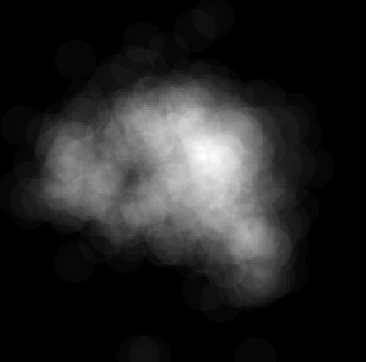
\includegraphics[width=0.25\linewidth]{./pics/saliency_map.png}& 
        
\includegraphics[width=0.25\linewidth]{./pics/2per.png}&
        
\includegraphics[width=0.25\linewidth]{./pics/5per.png}\\
        {\small  Saliency map} & {\small 2\% threshold} & {\small 5\% threshold}\\
     \end{tabular}
    \begin{tabular}{@{}c@{\hspace{0.1cm}}c@{}}
        
\includegraphics[width=0.25\linewidth]{./pics/10per.png}& 
        
\includegraphics[width=0.25\linewidth]{./pics/20per.png}\\
        {\small  10\% threshold} & {\small 20\% threshold}\\
    \end{tabular}
    \caption{A saliency map and its binary transformation following different thresholds}
    \label{fig:threshsal}
\end{figure}

\textbf{AUC-Judd}\\

AUC-Judd gets its name from the work of Judd and al. \cite{judd,Judd_2012,metricsreview}. For a given threshold the true positive rate is the ratio of true positives by the total numbers of fixations, true positives being values above the threshold at fixated pixels on the ground truth. False positives rate is also the false positives over the number of saliency map pixels at the given threshold. False positives are saliency values above the threshold at unfixated pixels in the ground-truth. \\

\textbf{AUC-borji}\\

From the Borji's work \cite{6751224} we get an other variant of AUC called AUC-Borji. The true positive rate is the same as AUC-Judd, but the false positive rate is the ratio of saliency map values above threshold sampled at random pixels (as many as fixations, sampled uniformly above the whole image), over the number of saliency map pixels at a given threshold. 


The last saliency maps AUC implementation is shuffled AUC \cite{sAUC}. It is meant to penalize models with a center bias.



\section{Chess expertise and eye tracking}\label{Chess expertise and eye tracking}


\textbf{Do an Introduction}


\subsection{Reingold and visual expertise}
Eyal Reingold is a Doctor in psychology who worked on perception and how chess players, depending on their expertise level, were looking at a chess configuration. In a paper from 2001 \cite{Charness2001},him and Charness discovered that experts compare to intermediate players, produce more fixations on empty squares. Also when fixating pieces, the number of fixations on relevant pieces was way greater. It was argued that experts were encoding configurations rather than pieces and produced patterns of saccading (quick movement of eyes between two or more phases of fixation).\\
In an other paper \cite{Perceptioninchess}, Charness and Reingold, demonstrated larger visual spans for expert players while processing structured chess positions. They also show that those experts player rather than fixating large number of pieces, would make fewer fixations and rather look at relation between pieces than on pieces. Finally an important idea that we can take from this work is that chess piece saliency influences the saccadic endpoints for experts making their encoding part faster than  intermediate players.\\
In a more recent paper  \cite{doi:10.1167/17.3.4} he presented the fact that chess expertise is mainly related to the detection of complex patterns and configurations. When improving our level, we become capable of detecting patterns in the pieces positions. This is why expert don't need to fixate pieces, and instead detect an interesting pattern by looking at its center.

\subsection{Using players level to aggregate their eye tracking data}
From the previous sub-section information we have an idea of how depending on the chess configuration and the player's level, the saliency map would look like. Taking only expert players and aggregating their data would give us very salient areas in the center of configurations and more focused on empty cells than on pieces as the Figure \ref{fig:fixationsempty} shows.\\
For intermediate players we should have a more spread salient area, including relevant pieces to the configuration. Adding less good players data, the salient area would concentrate toward pieces and would be more spread across the board, looking for "major" pieces such as queens,rooks,bishops...\\

\begin{figure}
    \centering
    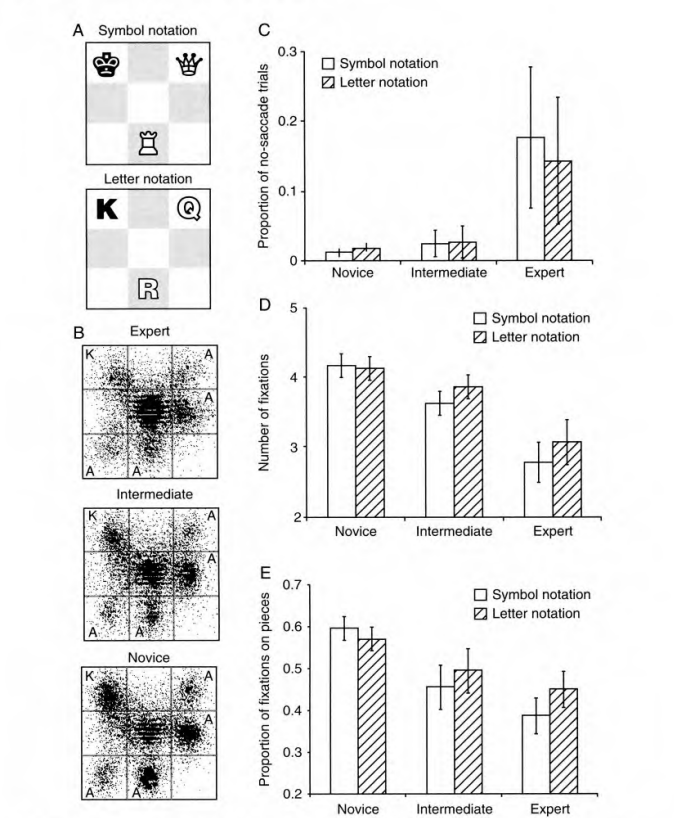
\includegraphics[scale=0.35]{./results/reingold_emptypieces.png}
    \caption{A figure on fixations of chess player from \cite{doi:10.1167/17.3.4}. In the left column we have the in A the notation of pieces and B the Scattergrams of gaze positions, for a check detection task (letter A represents an attacked piece position and K the king). In the right column we have the proportion of no-saccade trial (not moving the eyes from the center position and trying to solve the task), the number of fixations and the number of fixations on pieces for each level of players.}
    \label{fig:fixationsempty}
\end{figure}

Datasets in visual attention aggregate visual saliency maps of all users on images just by summing them up. This strategy, works pretty well since for images such as portraits or landscape, humans tend to look at them the same way and focus on quite similar points. As an example, a human face would be more salient around the eyes and mouth as this characterize us and make us see a face.
This way of aggregating data would work with chess, if our users would be only experts or intermediates. Otherwise just summing saliency maps would in the end create wide salient areas, not really characterizing human visual attention on the chessboard. We use instead an averaging method discussed later in the report ( section \ref{section:data}), taking at each pixels the average of values across the user.



    
    
\chapter{Method}
As mentioned in chapter \ref{SoA},human attention is defined such that we have two approaches which are bottom up and top down. 
In this chapter we first explain our main tool and our choices.
Then we are going to focus on the bottom up approach, using eye tracking data captured while chess player were playing games, training our network only on this data. Features are extracted and the network is learning how to produce visual attention map from them. 
Finally we will discuss how we started to think about the top down approach, which is leading visual attention based on the action we have to do. The conclusion being a quick overview of our implementation.


\section{Attention prediction Network and dataset}\label{section:model}
\begin{figure}[h!]
 \centerline{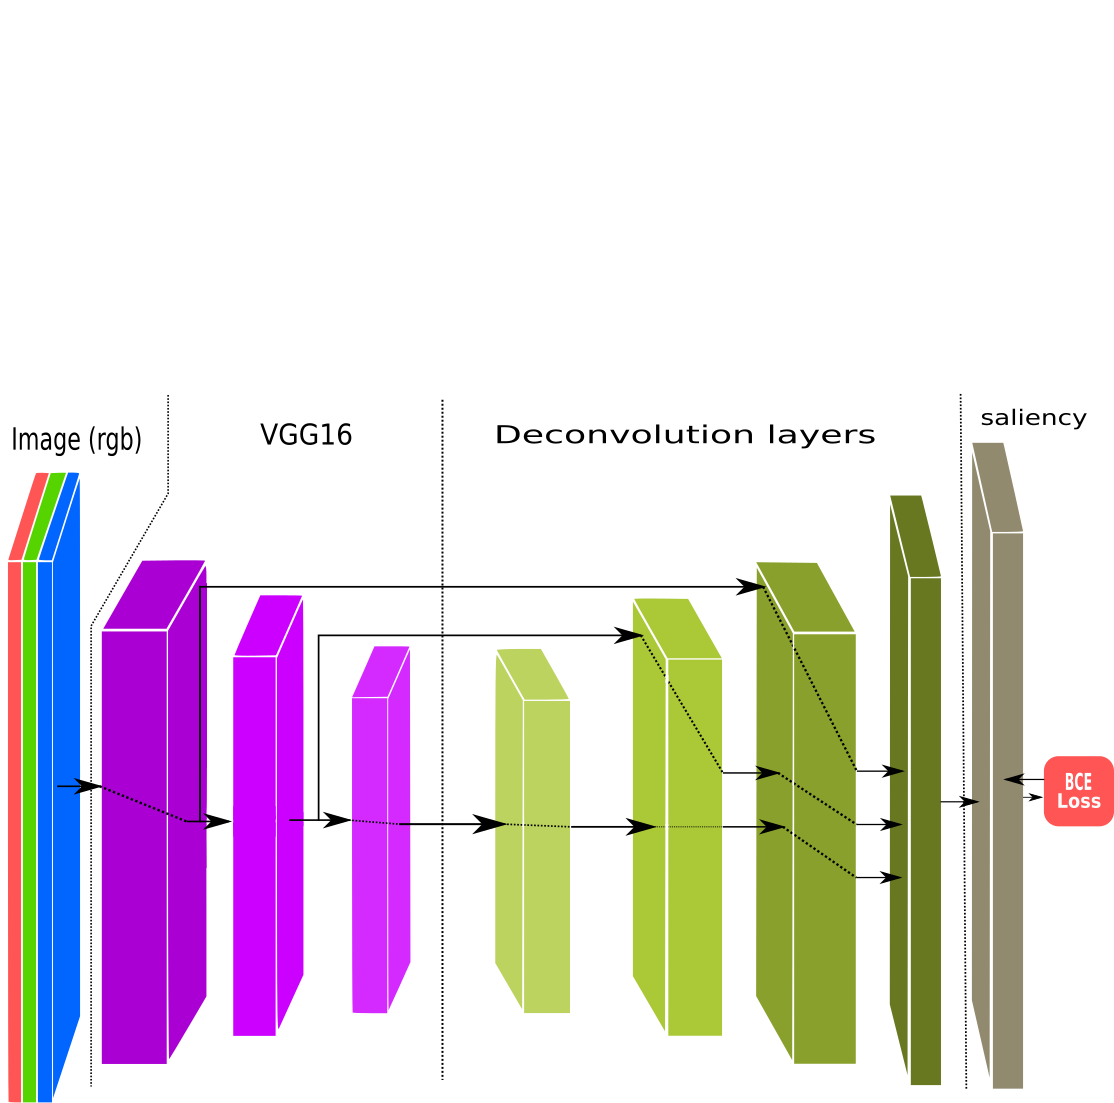
\includegraphics[scale=0.40]{./pics/network.png}}
 \caption{Our network}
 \label{fig:network}
\end{figure}
Our model presented in figure \ref{fig:network}, is inspired by the one used in Wang, and al. paper \cite{DBLP:journals/corr/WangS17b}. We use a multi-scale approach based on the skip-layer architecture, common in attention prediction. The first part (encoder) is the VGG16 \cite{DBLP:journals/corr/SimonyanZ14a} architecture, while the second part (decoder) is a succession of deconvolution layers stacked one on top of the others. The difference between our model and \cite{DBLP:journals/corr/WangS17b}, is that we share weights between these deconvolution layers. Their weights are initialized using a normal distribution, with a mean of 0 and a standard deviation of 0.01.


Sharing weights has several advantages. The first obvious one is the size of memory for deconvolution weights reduced by 5 in this case. The number of parameters to optimize is also reduced and thus the network is converging way faster.
We had also an other intuition behind sharing weights. Because we take features at different scale in the Encoder part of the network, outputs of those layers have different field of view. At a small scale, with a reduced field of view,let say of maximum 2 cells. If we have a bishop endangered by a pawn, translated as a local feature map, it is logical that this relation become salient in the final saliency map. Now if we take the same relation between the two pieces, but this time across the board, where the bishop can take the enemy pawn, the network should consider this to be salient the same way as before but at a larger scale/field of view. This is why a feature map, upsampled using deconvolution, should be deconvoluted using the same weights as an other feature map of the same dimensions.


The input of the network is a image encoded on three channels (Red, Green and Blue), resized to 224 pixels by 224 using bilinear interpolation. We could use inputs encoded on the gray scale only. However our network is based on transferring knowledge from previously trained VGG network \cite{DBLP:journals/corr/SimonyanZ14a}. This previous knowledge was acquired using features from colored images. We show in section \ref{section:pretrain}, how this knowledge transfer is important and thus why we keep an input encoded on three channels. The last layer of the network which is producing a saliency map of the size of the input image, is doing the following :
\begin{itemize}
    \item Crop the three outputs from the last convolution to the size of the input image (output shape :[3,224,224]) 
    \item Repeat them three times and stack them up (output shape : [9,224,224])
    \item Execute a final deconvolution on this stacked up data, to output a tensor of the shape [1,224,224]
    \item A Sigmoid function is applied on it to map the saliency values between 0 and 1.
\end{itemize}

All those steps end up giving us a saliency map, the same size of the original picture, encoded between 0 and 1.

\subsection{Deep learning layers}\label{Deep learning}

In this section we are going to describe few layers and methods we use in our model. Our model being based on convolution, we explain why using them and their principal components(Padding and stride) in section \ref{section:conv}. We then explain their counter parts name "deconvolution" and the pooling method. Finally we give a brief overview of Transfer learning and why using it in section \ref{section:transfl}.


\subsubsection{Spatial convolution}\label{section:conv}

Using a regular network such as a perceptron which is using only linear operations and activation function won't be a good idea when considering images. For example if we take a 300x300 rgb picture, we would need 2700001 parameters for a single neuron making the memory size of a network exploding. But images have spatial relationships which we can take advantage of, by convolving a set of N filters on the images creating  N 2D feature maps. Spatial convolutions are defined by the number of filter and the properties of the convolution (ie. padding and strides). \\

\textbf{Padding}\\

Padding is used to preserve information between convolutional layers and  the dimension of the output. Let say, we apply a 5*5 filter on a 32*32 input with a stride of 1, we would get an output of size 28*28, losing some information and quickly reducing the dimensions after few layers of convolution. For that we had some padding around the input to augment its dimension to 36*36,so that after the convolution layer the output keep the 32*32 dimension. Padding is simply adding some 0 values around the input. To keep the same dimensions with as stride of 1 the size of the padding is $p = \frac{k-1}{2}$ where k is the kernel size.\\

\textbf{Strides}\\

Strides control how we convolve the filter on the input. With a stride of 1 we move the center of 1 cell at a time, for a stride of 2, 2 cells at a time etc.. It allows to control the receptive field and how it overlaps.\\

\begin{figure}[ht!]
   \centerline{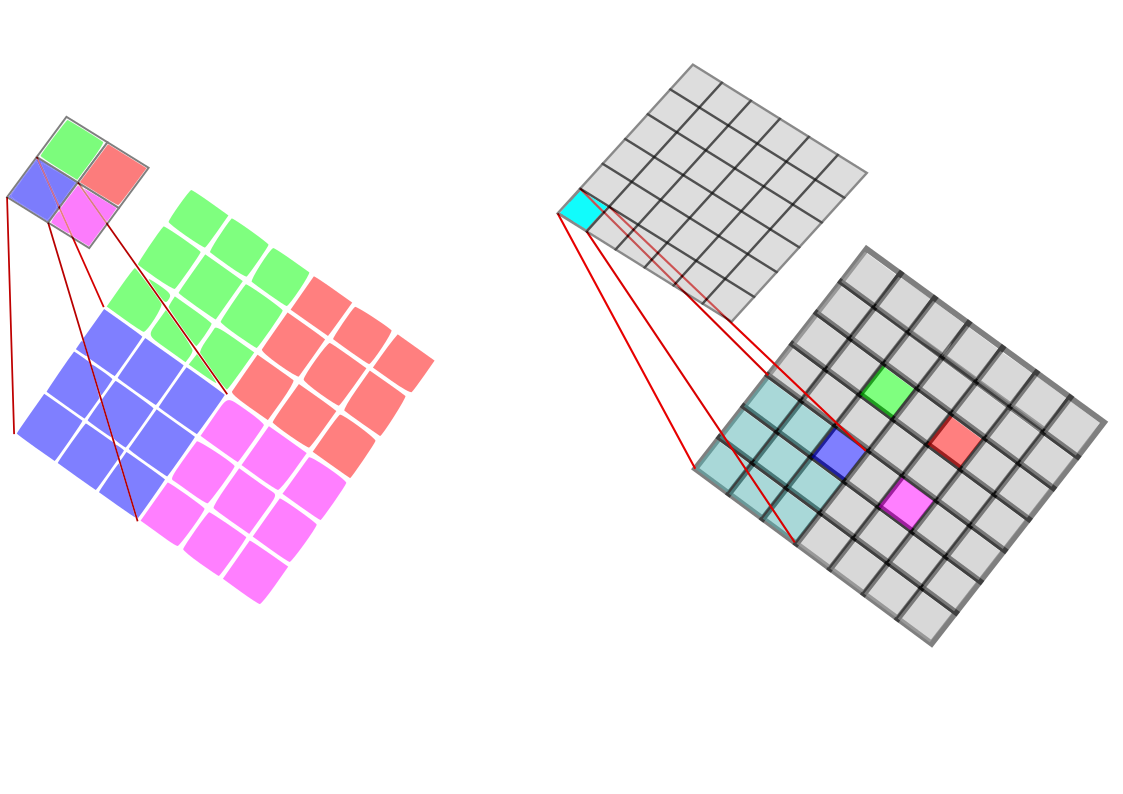
\includegraphics[scale=0.30]{./pics/convolution.png}}
   \caption{A convolution and its transposed counterpart}
   \label{fig:conv}
\end{figure}


The operation inverse to a convolution is a deconvolution, which is just basically reverting the operation done by a convolution.
In deep learning, deconvolution are not used but instead we use the Transposed Convolutions or fractionally strided convolutions which are wrongly called deconvolution. A deconvolution of an input 2*2 should get 9 values out of one for a previous convolution of a kernel of size 3 with a stride of 2. But because this would be a bit tricky, we instead do a simple convolution over the input, using some padding on it. The figure \ref{fig:conv} shows how a convolution is applied on an input and how the transposed convolution is computed on the result. The left part is the convolution applied on the 6*6 picture with 0 padding and stride of 2. The right part is how the transposed convolution is computed to get back to the original picture. A padding of two is added around the input and 0 values are inserted between the input values (because of the stride of 2).


\subsubsection{Pooling}

Pooling is used to reduce the size of the feature map by aggregating multiple cells in a single one, it also produce invariance to small variation between images. Several way of pooling exist such  as \textbf{Maxpooling} which is taking the maximum of the values in the area of the size of a filter, or \textbf{AveragePooling} taking the average instead. Figure \ref{}  illustrate pooling over a feature map.


\subsubsection{Transfer learning}\label{section:transfl}

Transfer learning start from the idea that features learned from huge amount of data, are relatively the same when looking at the first layers of Deep neural networks. Thus it if often not useful to retrain from scratch our network while we could start from already trained weights which can be pretty close to what the final weight of our network would be on our specific dataset. 
In their survey paper \cite{Pan:2010:STL:1850483.1850545}, Pan an al., worked on categorizing, explaining and discussing advancement on transfer learning up until 2009. Offering a broad explanation on techniques and work done on this part of the deep learning field.


\subsection{Data pre-processing}
The data given as an input to our network does not need a lot of pre-processing other than being re-sized and cropped to be just the size of a chess board. On the other hand some work needed to be done on the ground truth data being heatmaps from eye tracking data. The heatmaps were produced by an eye tracking software (Tobii Studio 3.4.7) which was simply doing a convolution of colored Gaussian on user's fixations. The problem was that the color scheme use for those Gaussian was not directly transformable to grey scale data by taking the average of the three channels Red Blue and Green. Figure \ref{fig:gray} Shows a heatmap taken from the eye tracking software and converted to grayscale.\\

\begin{figure}[ht!]
    \centering
    \begin{tabular}{c@{\hspace{0.2cm}}c@{\hspace{0.2cm}}c@{\hspace{0.2cm}}c}
    
        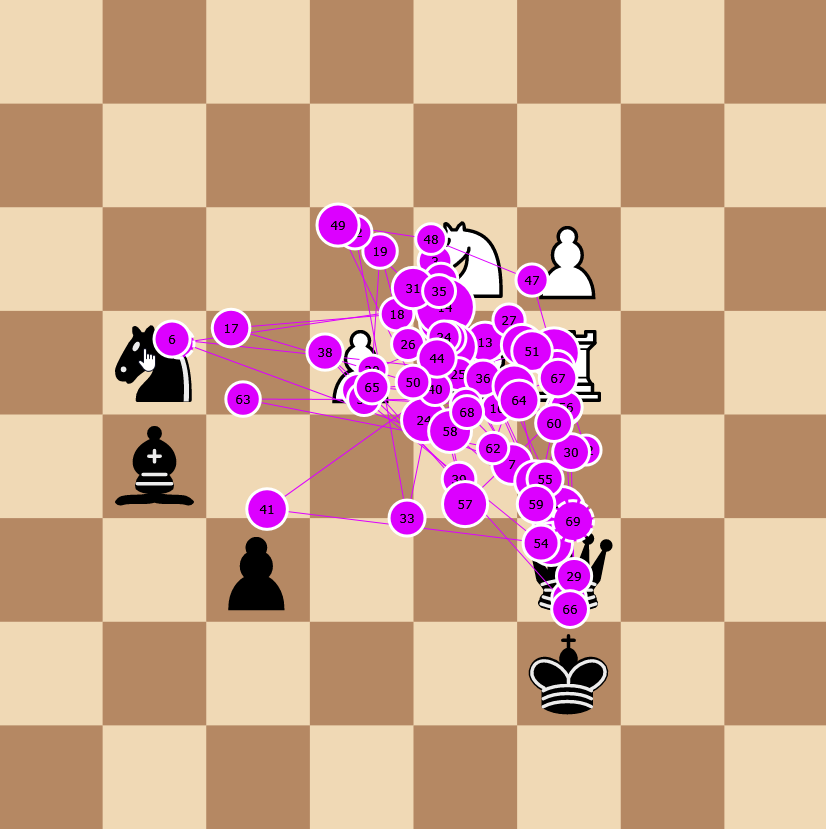
\includegraphics[width=0.25\linewidth]{./transformations/origin.png}& 
        
\includegraphics[width=0.25\linewidth]{./pics/base_image.png}& 
        
\includegraphics[width=0.25\linewidth]{./pics/color_to_gray_wrong.png} & 
        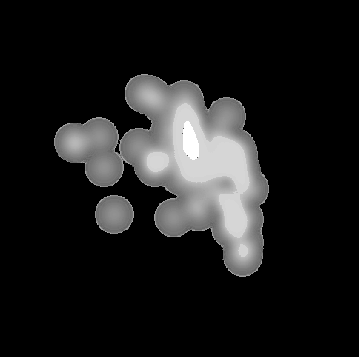
\includegraphics[scale=0.313]{./pics/correct_gray.png}\\
        {\small  Scan path} &{\small  Heatmap} & {\small Gray scale conversion (A) } & {\small A correct representation (B)}\\ 
        {\small  } & {\small  } & {\small  by averaging} & {\small of gray scale}\\ 
         {\small  } &{\small  } & {\small  } & {\small }\\ 
    \end{tabular}
    \caption{From scanpath to heatmap to incorrect gray scale representation (A), and correct gray scale representation (B)}
    \label{fig:gray}
\end{figure}
The solution was to create ourselves the translation from Red Blue and Green encoding to a gray gradient between 0 and 1. Red (encoded as [255,0,0]) became 1, decreasing through orange  ([255,>128,0]) and yellow ([255,255,0]), to light green ([0,255,0]) and darker Green ([0,>150,>50]. Taking in consideration the value of Green for closer to red colors and Blue for color closer to green, allowed us to create a gradient representation as in figure \ref{fig:gray} (contours of Gaussians being brighter than the inside is due to a bug from the eye tracking software, which is adding lighter green to the exterior of  Gaussians).

Our model is close to a standard auto-encoder architecture which basically learns to encode some data and to decode it to be like the input. The logic way to compare its output to the input would be to compute the distance between them and to minimize it. 
For that there is the basic, simple and intuitive L1 loss, being $|y - f(x)|$ (with y as the GroundTruth and f(x) the output of the auto-encoder), could be a solution. We also have the L2 loss, also known as Mean square error express as $ (y- f(x))^2$.

But in our case we don't learn how to generate a copy of our input being a chessboard with pieces on it, but the visual prediction of this chessboard. The visual prediction is a probability distribution between 0 and 1, 0 being not looked at at all (black) and 1 long fixations (white) (or salient or not salient).
In statistics the Kullback Leibler divergence \cite{10.2307/2236703} express how much two probability distributions are diverging one from the other, minimizing it is equivalent to reducing the distance between them. 
It can be expressed as the equation \ref{eq:KL}.
\begin{equation}
    \label{eq:KL}
    KL(P|Q) = \sum\limits_{i=1}^n P(i) \frac{P(i)}{Q(i)}
\end{equation}
However Kullback Leibler divergence is not a metric as it doesn't respect the triangle inequality and often $KL(P|Q) \neq KL(Q|P)$. But if we develop the expression of equation \ref{eq:KL} in \ref{eq:devKL}:

\begin{align}
\label{eq:devKL}
KL(P|Q) & = & \sum\limits_{i=1}^n P(i) \frac{P(i|x)}{Q(i|x)}\\  
& = & \sum\limits_{i=1}^n ( - P(i|x) log(Q(i|x))  + P(i|x) loq(P(i|x)))\\
& = & - \sum\limits_{i=1}^n   P(i|x) log(Q(i))  + \sum\limits_{i=1}^n P(i|x) loq(P(i|x))\\
& = &  -\sum\limits_{i=1}^n  P(i|x) log(Q(i|x)) - \sum\limits_{i=1}^n P(i|x) loq(\frac{1}{P(i|x)})\\
&  = & -\sum\limits_{i=1}^n   P(i|x) log(Q(i|x)) - H(P(i|x))
\end{align}

If we take our Ground truth as P, because it doesn't change its entropy is equal to 0 and we have just the cross entropy between our two probability distributions $ -\sum\limits_{i=1}^n   P(i) log(Q(i)) $
Taking a binary approach, with i being either 0 or 1 (salient or not salient), $Q(i|x) = y$ our Ground-truth  and $P(t|x) = c$ the output of our model, we can write $-\sum\limits_{i=1}^n   P(i|x) log(Q(i|x)) - H(P(i|x)) = -ylog(c) - (1-y)log(1-c) $, giving us the formula of the Binary Cross entropy. 
We show that binary cross entropy in the case of saliency map generation can be seen as relatively close related to the Kullback Leibler divergence. Minimizing it would allow us to generate data as close as possible to the groundtruth.

Also we will no use Kullback Leibler divergence as a metric in this report for several reasons discussed in \cite{LeMeur2013} and \cite{metricsreview} among other paper cited in this report. The first one being that this distance is non-linear, non-symetric and it doesn't respect the triangle inequality. Also the fact that there is no upper bound clearly defined is a problem. This distance between two generated saliency maps and a groundtruth, gives us an overall dissimilarity and allows us to see which one of the saliency maps has the highest.

\subsection{Dataset}
\subsubsection{Available data} \label{section:data}
The data we started with comes from the experiments of Thomas Guntz \cite{thomasguntz}. He worked on the multimodal study of people solving various problems and in particular chess problems. For his experiments he recorded the eye-gaze of several players from various level, trying to solve different chess task of increasing difficulty (from openings to king in check in N moves). There were 11 configurations (Figure \ref{fig:dataset}) on which  were captured around thirty players eye tracking data. Because visual attention is quite subjective and even if it depends on the chess player level, it often has some divergences. For that we decided to group all our heat-maps into one saliency map, being the average of them. Why the average? Because we didn't have the  same amount of people in the "expert" category than in the "amateur" one. Hence areas where the expert would focus wouldn't have been a good representation of the areas player often looks at. Averaging all those heat-maps we get a good idea of areas which are important for most of the players, those being less important are darker in the gray scale.

 \begin{figure}[ht!]
    \centering
    \begin{tabular}{@{}c@{\hspace{0.2cm}}c@{\hspace{0.2cm}}c@{\hspace{0.2cm}}c@{}}
        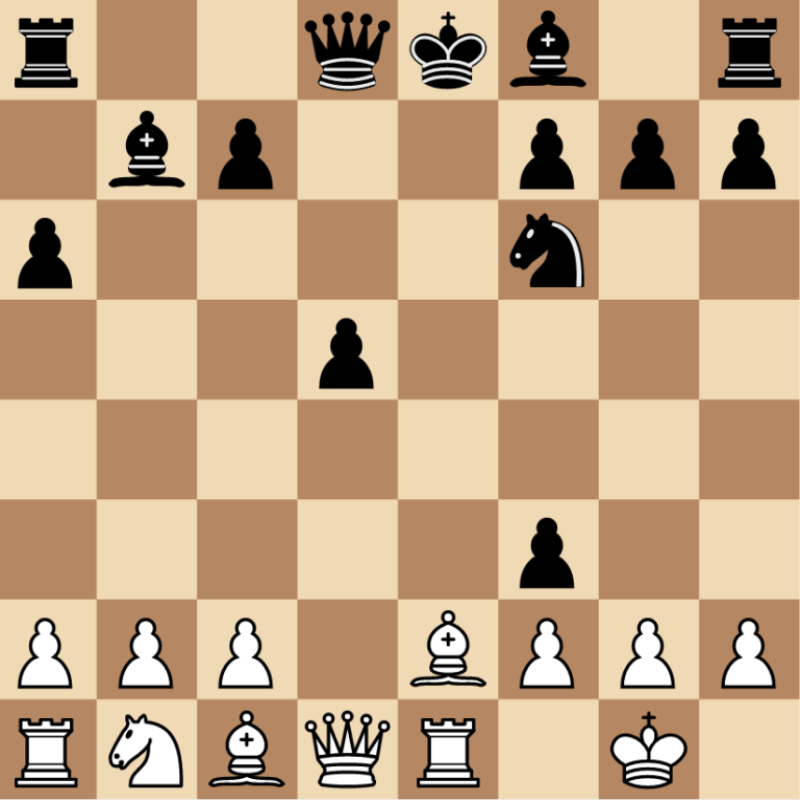
\includegraphics[width=0.25\linewidth]{./dataset/configIV.png}&
        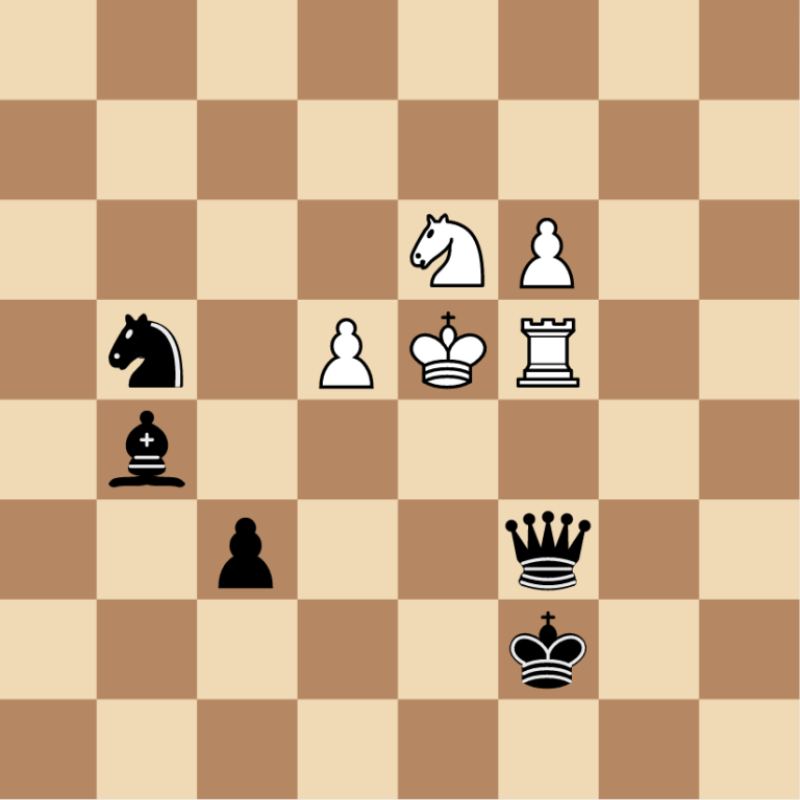
\includegraphics[width=0.25\linewidth]{./dataset/configIX.png}&
        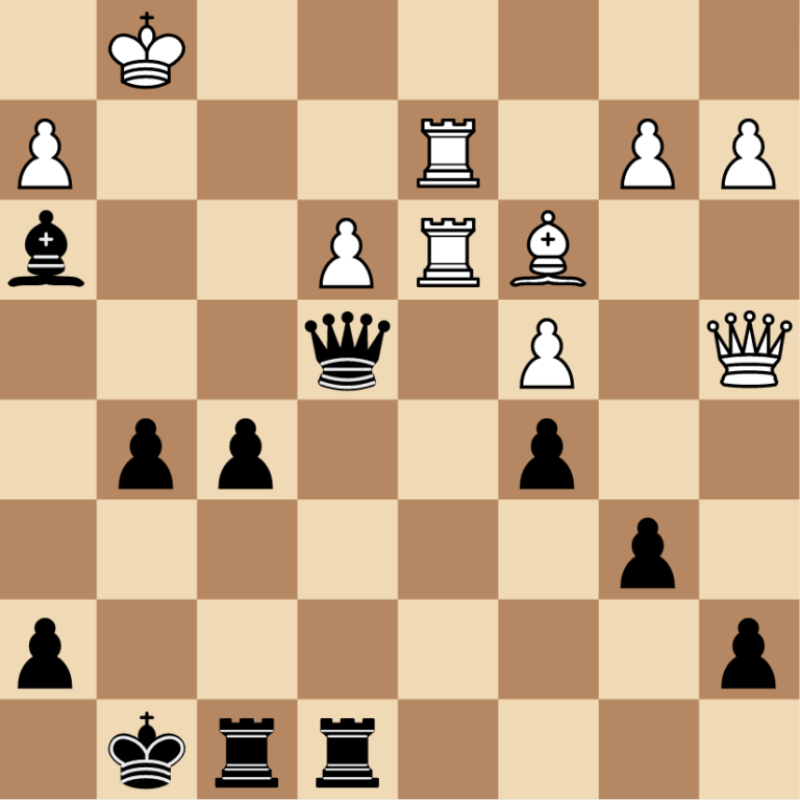
\includegraphics[width=0.25\linewidth]{./dataset/configLI.png}&
        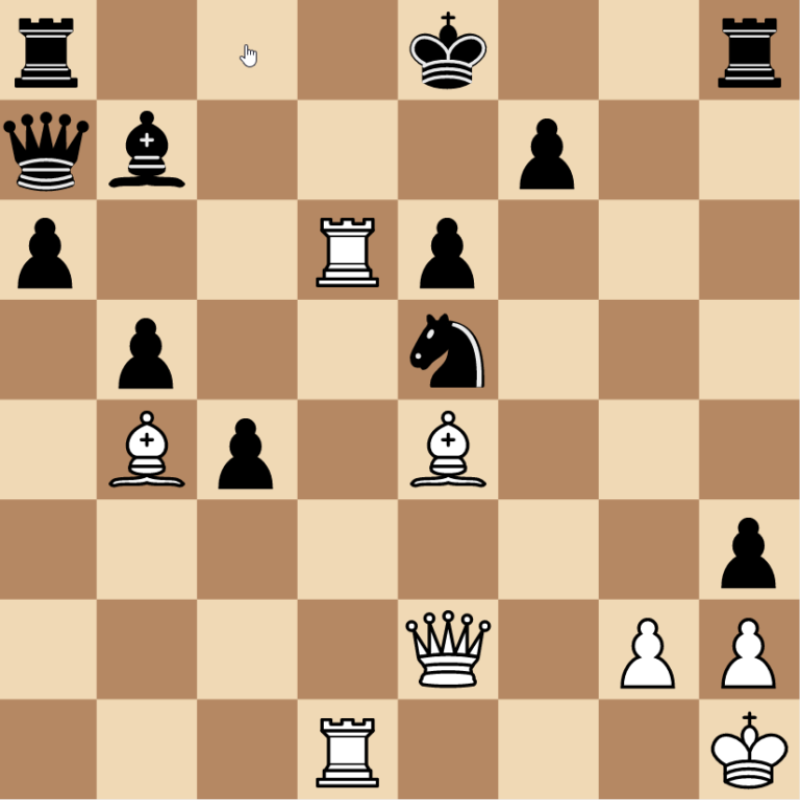
\includegraphics[width=0.25\linewidth]{./dataset/configLIX.png}\\
        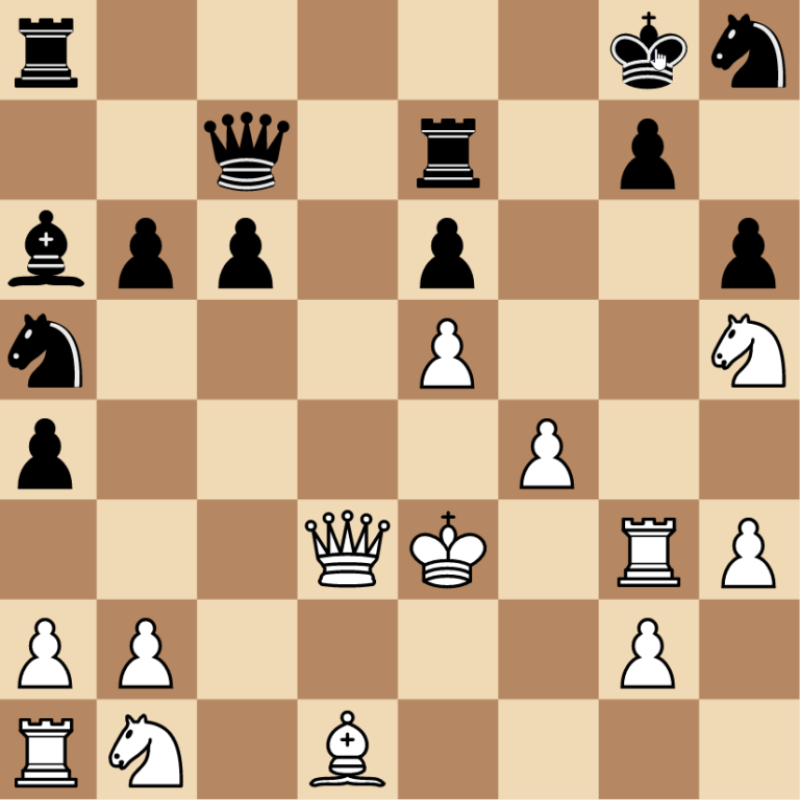
\includegraphics[width=0.25\linewidth]{./dataset/configLXIX.png}&
        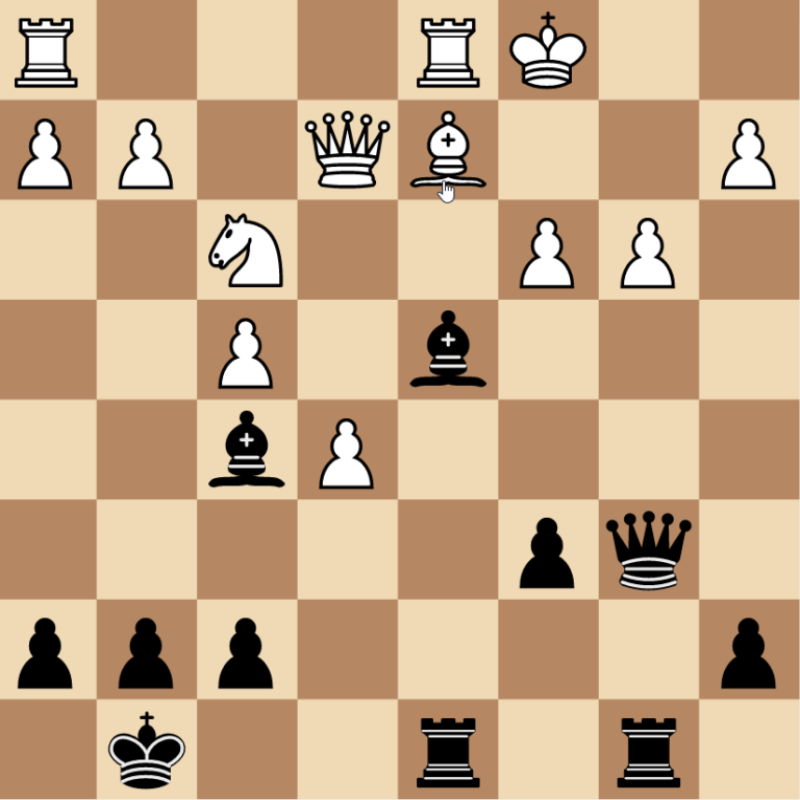
\includegraphics[width=0.25\linewidth]{./dataset/configLXVII.png}&
        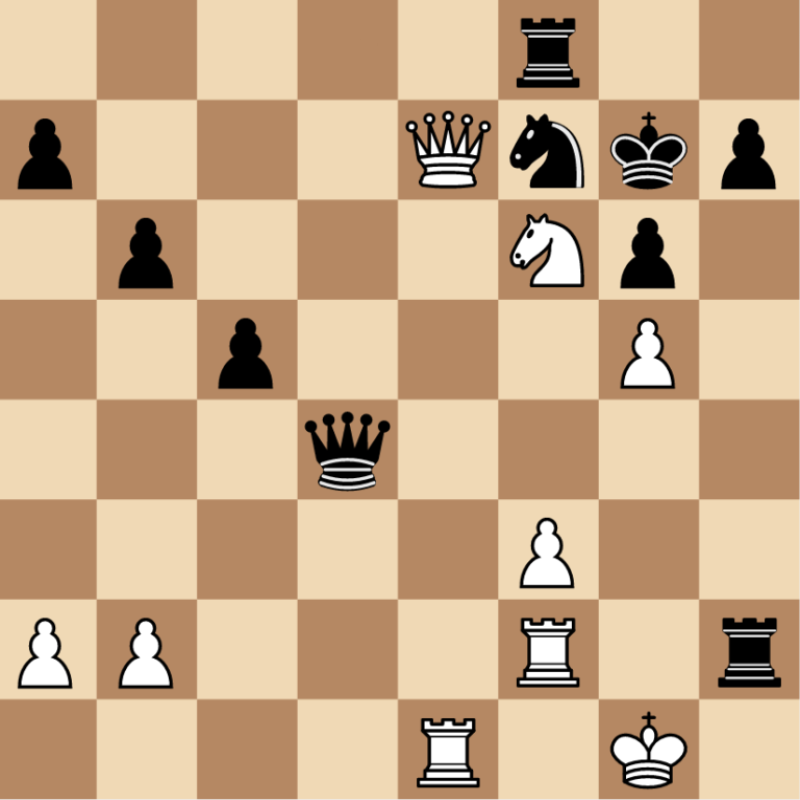
\includegraphics[width=0.25\linewidth]{./dataset/configRXLII.png}&
        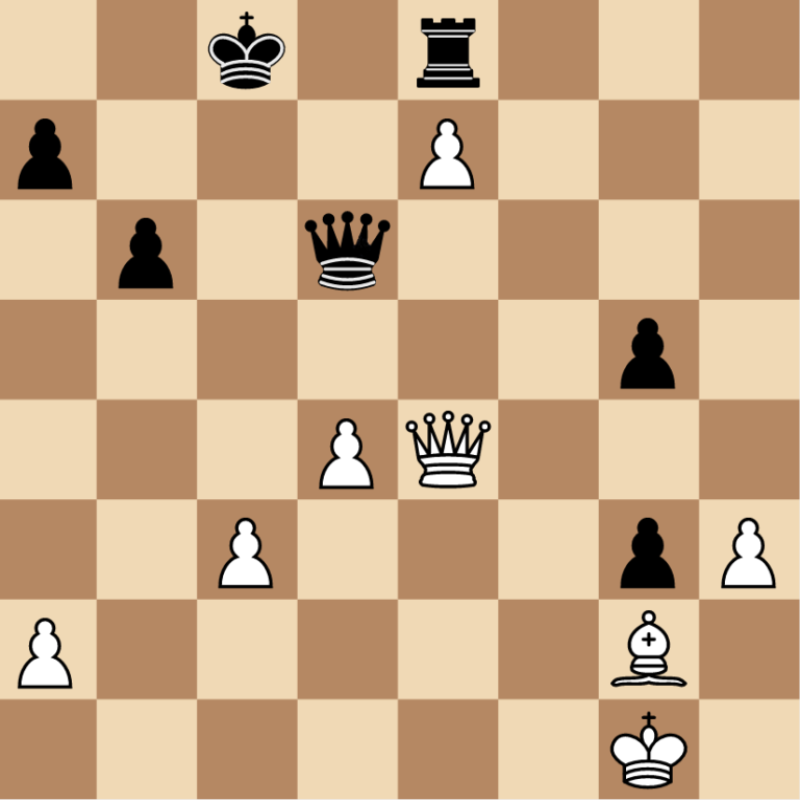
\includegraphics[width=0.25\linewidth]{./dataset/configV.png}\\
    \end{tabular}

     \begin{tabular}{@{}c@{\hspace{0.2cm}}c@{\hspace{0.2cm}}c@{}}
        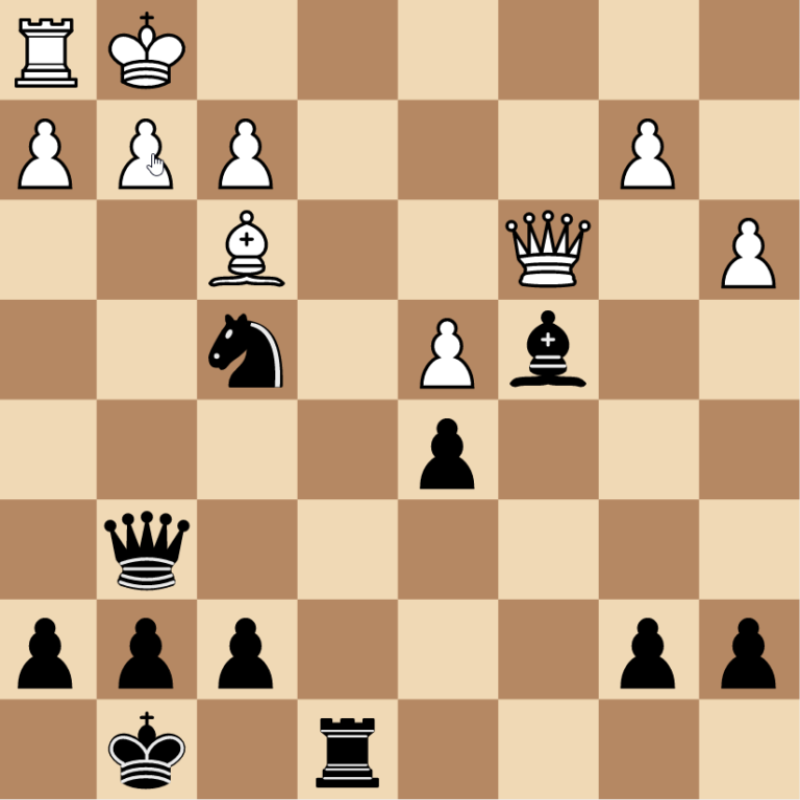
\includegraphics[width=0.25\linewidth]{./dataset/configXVI.png}&
        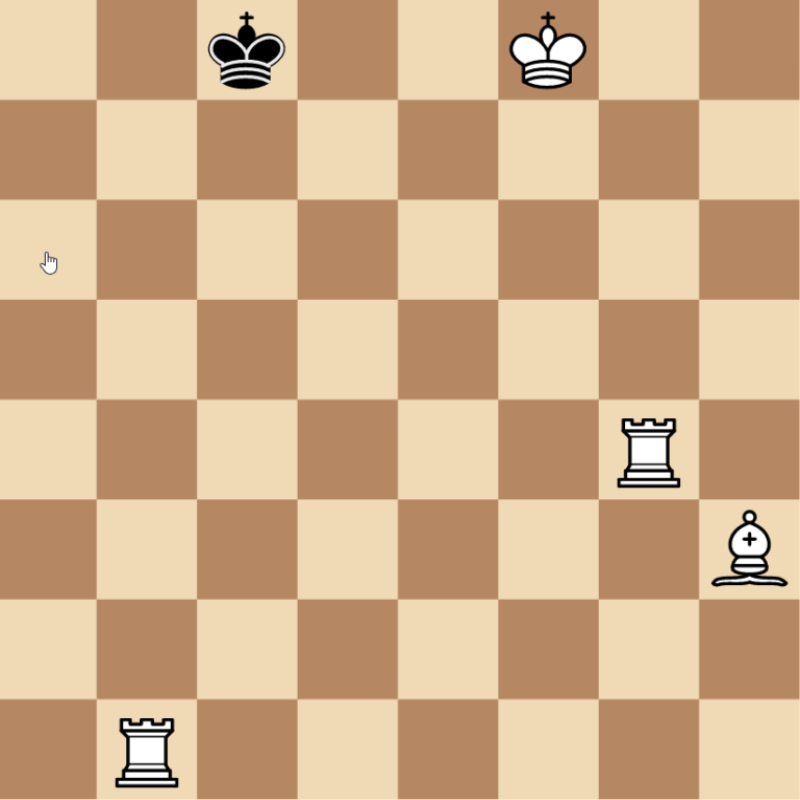
\includegraphics[width=0.25\linewidth]{./dataset/configXVII.png}&
        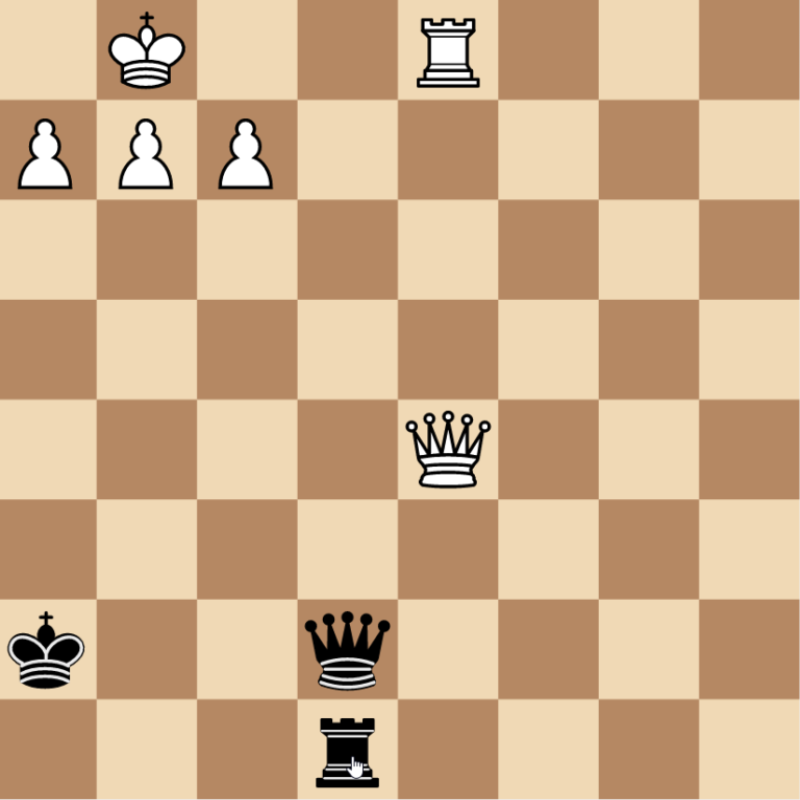
\includegraphics[width=0.25\linewidth]{./dataset/configXXIX.png}\\
       
    \end{tabular}
    \caption{Our dataset}
    \label{fig:dataset}
\end{figure}
    

Also as we mentioned when talking about Reingold  and al. work \cite{doi:10.1167/17.3.4,Charness2001}, "expert" players tend to look at the center of important configuration. When averaging players's eyetracking data we noticed than "expert" fixations were positioned on the most salient part of the saliency map, where most people were looking at, despite not being the most representative part of the players we had.

This little prepossessing done, we end up with 11 configurations and the same amount of saliency maps.
With such limited data, we needed ways to augment it while keeping data interesting and relevant.
\subsection{Data augmentation}
Data augmentation is the act creating variations of the dataset, to multiply the examples the network will learn on and help him generalize even more its knowledge to more and more complex examples. This include many transformation such as rotation, translation, flipping the image, scaling, cropping a part of the image , or even adding some noise to it to add some difficulty.

    \subsubsection{Cutting  board}
    The first augmentation we could think of was cutting the board into smaller pieces, same thing for the corresponding saliency map. So we could force the network to focus on specific parts of the board and learn how to look at those. We started with cutting it in four "4x4" part each being a quarter of the original board. We then thought about cutting in three by three  and five by five parts. But those being odd numbers of cell we needed to do the convolution of this cutting over the board on row and one column at a time. Doing that we had multiplied the amount of data by 150.
    \begin{figure}[ht!]
    \centering
    \begin{tabular}{@{}c@{\hspace{0.4cm}}c@{}}
        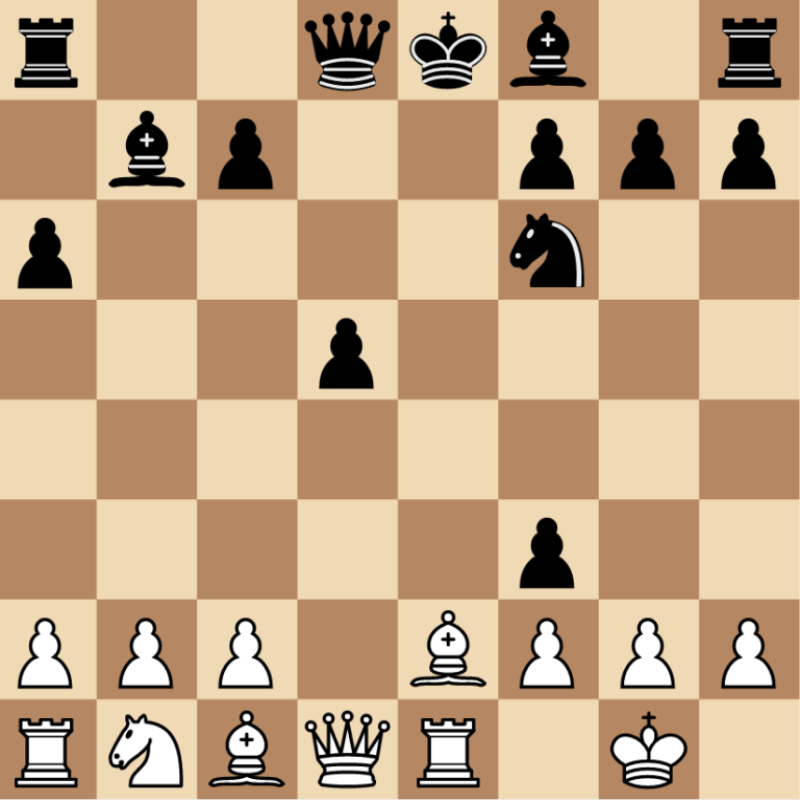
\includegraphics[width=0.25\linewidth]{./transformations/config.png}&
        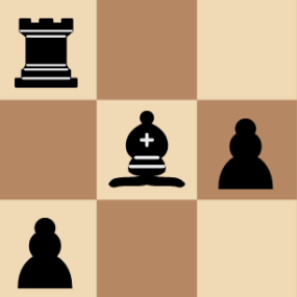
\includegraphics[width=0.25\linewidth]{./transformations/3.png}\\
        {\small  Configuration reference} & {\small Cutting in 3*3 cells}\\
         {\small  } & {\small }\\
        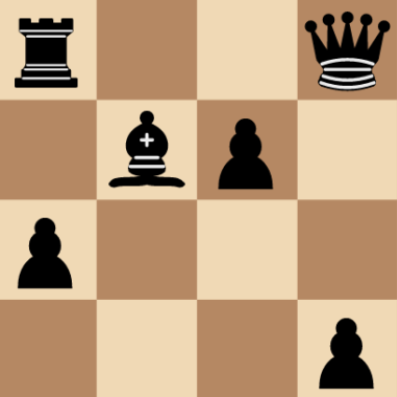
\includegraphics[width=0.25\linewidth]{./transformations/4.png}&
        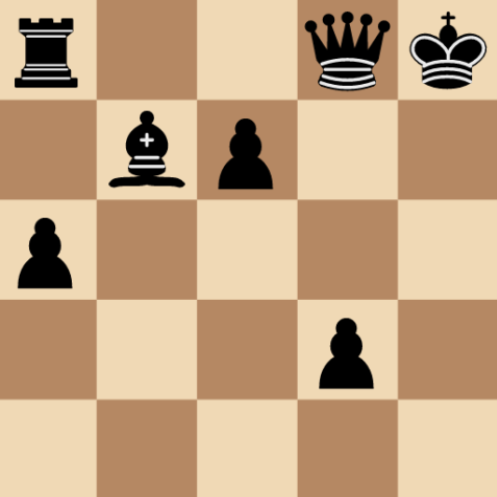
\includegraphics[width=0.25\linewidth]{./transformations/5.png}\\
        
        {\small  Cutting in 4*4 cells} & {\small Cutting in 5*5 cells} \\
         {\small  } & {\small }\\
    \end{tabular}
    \caption{Configuration and how it we cutted it}
    \label{fig:cutting}
\end{figure}
    
    \subsubsection{Pieces color inversion}
     An other augmentation was to invert the color of each piece (black to white and white to black). Because every configuration is possible while playing white and black, inverting colors was adding diversity of configurations the network could see. 
     To do that we used a neural network trained to classify chess pieces, we just needed to identify the cell color to replace the piece on each cells.
     \begin{figure}[ht!]
    \centering
    \begin{tabular}{@{}c@{\hspace{0.4cm}}c@{}}
        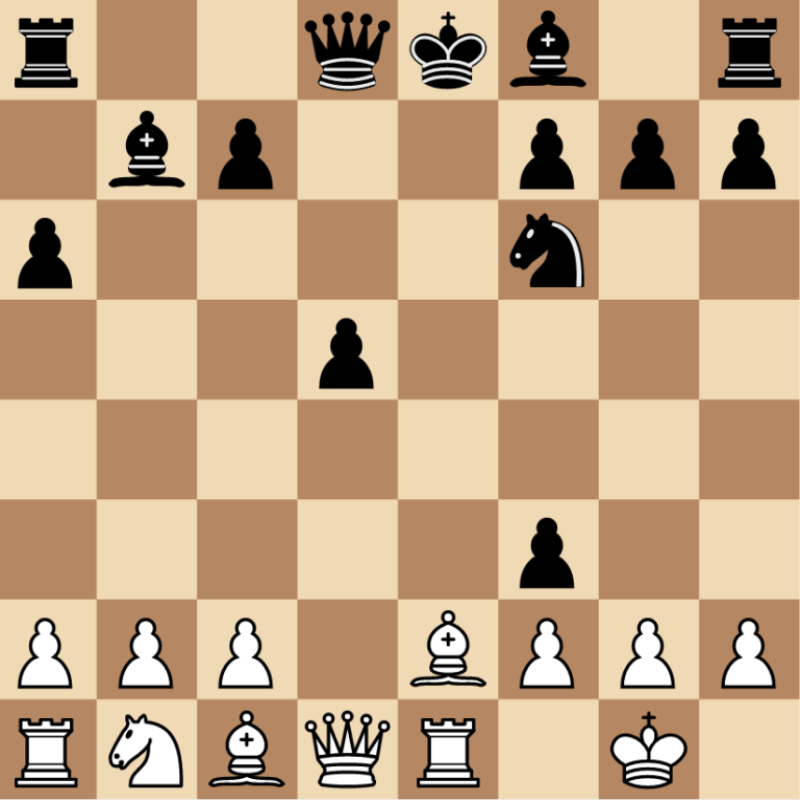
\includegraphics[width=0.25\linewidth]{./transformations/config.png}&
        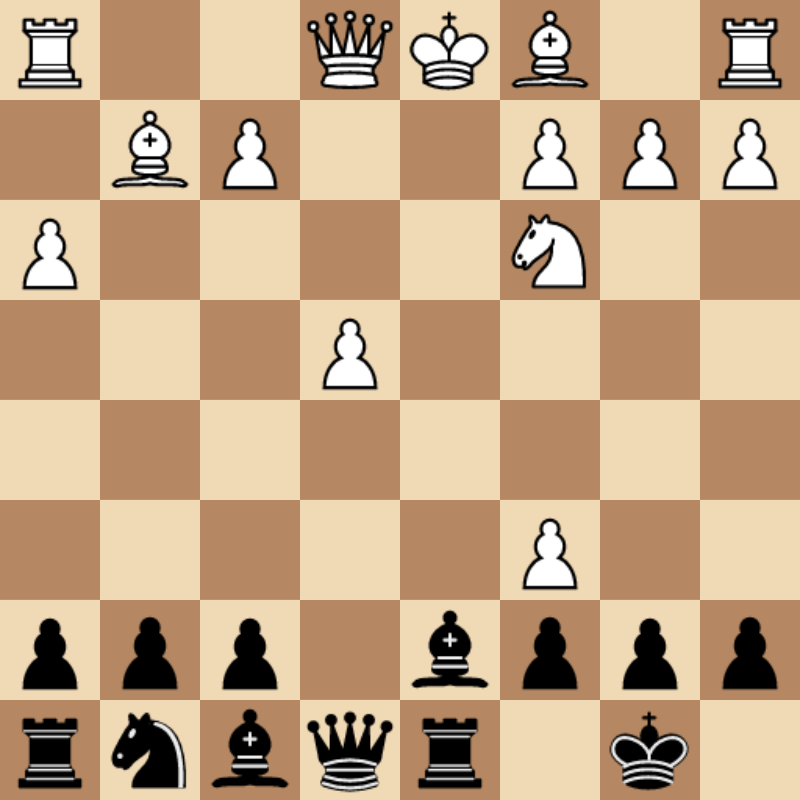
\includegraphics[width=0.25\linewidth]{./transformations/inverted.png}\\
       
        {\small Reference configuration} & {\small Same configurations } \\
        {\small} & {\small  inverting colors } \\
         {\small  } & {\small }\\
    \end{tabular}
    \caption{Configuration and its inverted counterpart}
    \label{fig:cutting}
\end{figure}
     
    \subsubsection{Flipping board}
    The last augmentation we used is  to change the orientation of the board, to the point of view of the other player. We considered that at any point of time, a chess player exploring his adversary possibilities would look at the board the same way he does. 
    
    \begin{figure}[ht!]
    \centering
    \begin{tabular}{@{}c@{\hspace{0.4cm}}c@{}}
        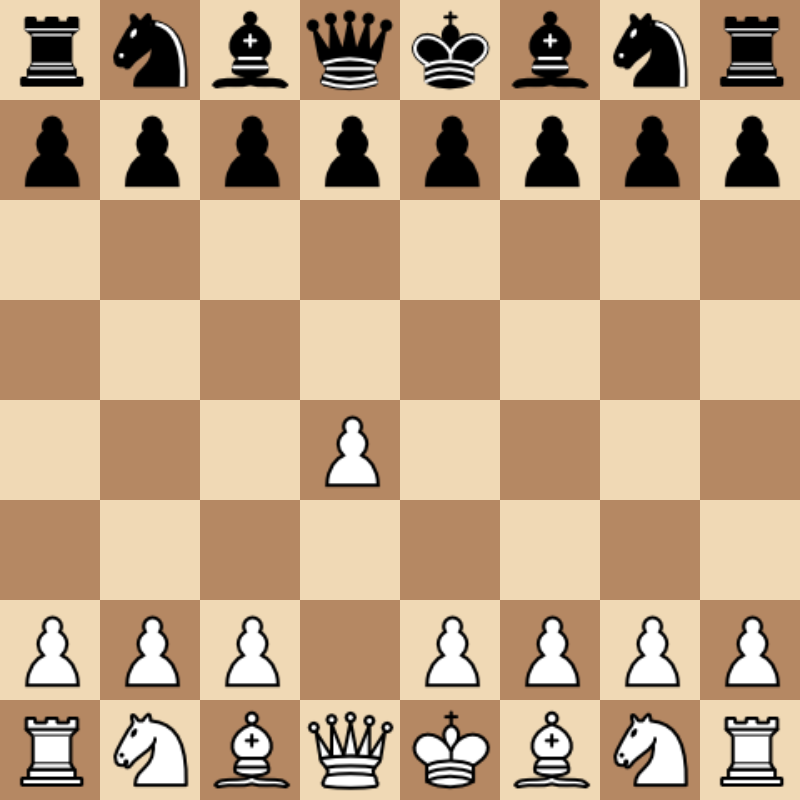
\includegraphics[width=0.25\linewidth]{./transformations/one_side.png}&
        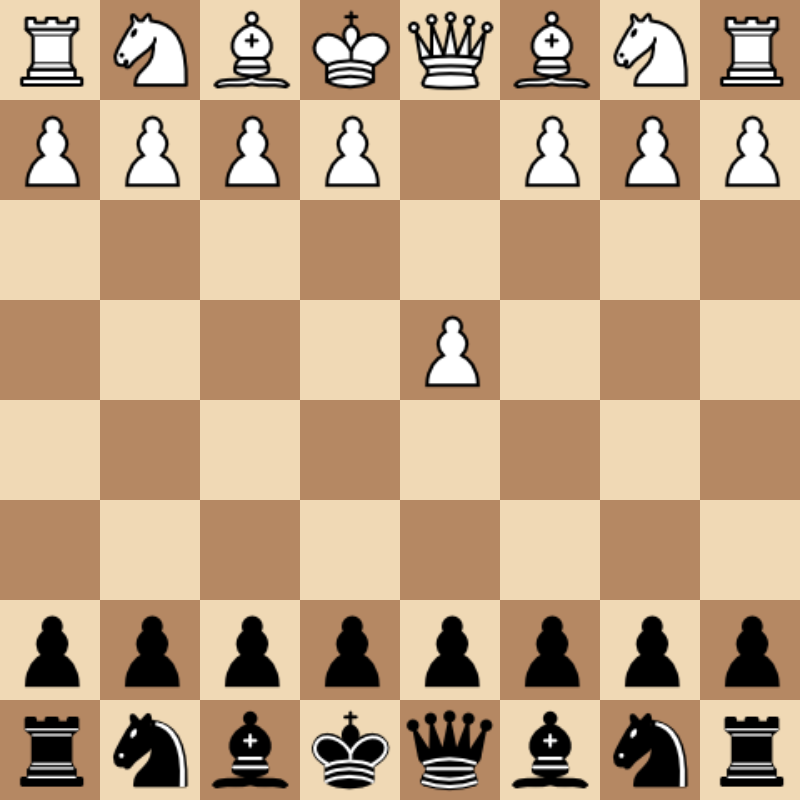
\includegraphics[width=0.25\linewidth]{./transformations/other_side.png}\\
       
        {\small Reference configuration} & {\small Same configurations  } \\
        {\small } & {\small  from enemy point of view} \\
         {\small  } & {\small }\\
    \end{tabular}
    \caption{Configuration and its inverted counterpart}
    \label{fig:cutting}
\end{figure}

\subsection{Training}

Training a deep neural network in an efficient way, as teaching a young child is not an easy and well defined process. Even though the algorithm is defined, its hyper parameters such as learning rate and how to set them, is very difficult and task dependant, requiring some prior thinking and attempts.  
For our problem we faced some difficulties concerning the learning rate and how to train using our data.


\subsubsection{Learning rate} 
Learning rate is one of the most important hyper-parameter when talking about training neural networks in an optimal way.
The bigger the learning rate is , the faster the weight will decrease toward a local minimum, but not necessarily to a good minimum.
That is why setting the learning rate to a value not too big to avoid some false minimum, but no too little to avoid too long training time. In his paper Leslie N. Smith \cite{DBLP:journals/corr/Smith15a} propose a cyclical learning rate, accelerating convergence toward a better accuracy than with a standard modification of learning rate. We use this strategy and compared it to the standard strategy of making the learning rate decrease after a certain amount of epochs. The learning rate was set at a maximum of 0.01 and a minimum of 0.0001.

\subsubsection{Using some prior training}

Even though the encoder part of our network is already trained and has his weights set for some features of Imagenet dataset \cite{imagenet_cvpr09}, the decoder part is at the beginning randomly initialized. The idea behind training our network on some other dataset before our own, is to initialize the decoder part to make it learn to transform features to salient or not part of the final saliency maps. 

Our first idea was to train it on the CAT2000 dataset \cite{DBLP:journals/corr/BorjiI15}, a dataset created by Borji and Itti, of about 4000 images for 20  different categories and 24 observers per images. The saliency maps of this dataset are created by convolving Gaussian of size  of 38px (size called degree of visual angle, DVA).

The second idea was to use the data created as described in then next section as this data would be more relevant to the chess problem.

\subsubsection{Training phases}

To avoid training a model for 10 days while it wasn't learning anything from the start, we made our training process as much explicit and easy to test as possible. Every 50 epochs a version of the model was saved and tested to visualize its progress. Loss was also monitored continuously. Various way of decreasing learning rate were tested. The main one which was considered as the most efficient was to train the network two thousands epochs at a time, and by looking at the loss for the last 100 epochs we decided or not to decrease the learning rate.

\section{Leading the network to learn tasks}

Top down approach in visual attention prediction is looking for relevant information in a picture depending on the task we have to accomplish. In chess the task is well defined as it is to move at a time T and for a specific configuration, the piece that is satisfying the most the condition which is : to win the game.
Because we are working with visual attention and saliency maps, we decided not to train a network to play chess (like Alphazero \cite{DBLP:journals/corr/abs-1712-01815}) and generate saliency maps depending on the pieces it considers to play at each round, but to create data leading the network to learn important pieces for a given configuration.

\subsection{Creating the data}
\subsubsection{Getting the configuration}
Since the beginning of the project we worked with Lichess \footnote{\url{https://en.lichess.org/} (last seen 06/2018)}. This online and offline chess platform allows to create personalized game and to play against other player or AI. With thousands of players registered and millions games played every month this is a gold mine to get data from. They even give access to a monthly database giving in the PGN format, all the games played during the past month. As an example for the month of March more than 22 million games have been played on this platform, giving us a quite big text file of 5 GB. Just with this file we would have enough data and nearly every used combinations in chess.

\subsubsection{From text to pictures}
From the beginning we have worked using screen capture of a chess game played on Lichess as an input for our network (the ground truth/target being a eye gazing heat map). So we needed to convert all the games we had to images to feed to our network.

PGN is a format giving for each turn the move done by white and black. Every move is based on the configuration of the board before the move and in the beginning black and white on their side of the board. Moves can be encoding as simple as two characters as "e4" for a pawn moving to e4 from e2. Or in a more complex way as "Nbxc3" for a knight moving from b2 and capturing a piece in c3. 
Without going into more details, what we needed to do was to create a parser to PGN format taking into account the complexity of the notation to create images from few lines of text. 

Once this done, we got from thousands of games, thousands of corresponding images.

\subsubsection{From a move to its heat map}

Because creating eye gazing data without an eye tracker is not really possible or would take a long time and wont be really objective, we needed to find a way to fake it while creating meaningful data. 
The idea we got was that a player when moving a piece looks at its destination and where it comes from. Even if it doesn't include the ultimate goal of a player when he is moving the piece (putting the enemy king in check or threatening a enemy's piece), it gives at least and idea on small areas and directions the player looks at.\\ 

\textbf{End and start points}\\

The first things we need to put as salient region are the start and end cells. We use for that a Gaussian shape a bit smaller than a cell, to represent a strong fixation.\\ 


\textbf{Trajectory}\\

From the origin and destination of a piece during each turn we would get two salient point, and adding the trajectory of the piece , we would get the path taken by the eye. This salient area is less bright than the end and start point as it doesn't correspond to long and strong fixations, but rather short and quick saccades. \\ 


\textbf{King in check}\\

We can also add the enemy king as a fixated point as when the move played is meant to put this king in check, we can consider that this piece is fixated by the player.\\ 

Figure \ref{fig:examplesconf} shows how a move can be transformed into a saliency map.

\begin{figure}[ht!]
    \centering
    \begin{tabular}{@{}c@{\hspace{0.1cm}}c@{\hspace{0.1cm}}c@{}}
        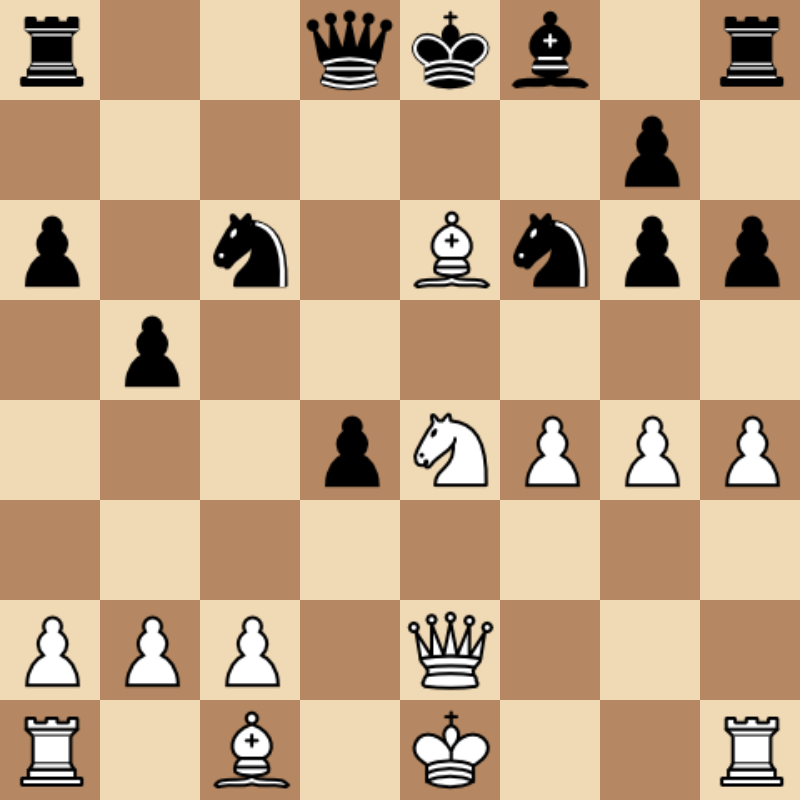
\includegraphics[width=0.25\linewidth]{./pics/config1.png}& 
        
\includegraphics[width=0.25\linewidth]{./pics/saliency1.png}&
        
\includegraphics[width=0.25\linewidth]{./pics/bishopmove.png}\\
        
        {\small  Configuration reference} & {\small Salient points } & {\small The salient trajectory }\\
        {\small  Configuration reference} & {\small  (start, end, check)} & {\small  for a bishop}
    \end{tabular}
    \caption{Configuration and saliency map we can generate from it}
    \label{fig:examplesconf}
\end{figure}


\subsubsection{Final data}\label{section:descpnewdataset}

After all those steps we got a bigger dataset than what we were working with before. With around two thousands games and an average of fifty round each, giving us a bit more than one hundred and twenty thousands images that we can use as training data. Also this dataset was extensible as much as needed. Because we got our data from an opensource database containing Billions and Billions of games from thousands of players, the amount of data we could add to the dataset was quite huge. But we still limited the size of the dataset, to be able to train a minimum amount of epochs on it and because the generation of data, even in parallel was taking quite some time because of the disc operations when creating images.


Even though this new dataset was consequent and rich enough, some biases were still present.
The first one was that even with the large amount of configuration created, the vast majority of them were openings and their number being limited, there were a lot of redundancies.
The second bias was subjectivity of the saliency maps created. And the last one was the pieces moved compared to the number of pieces for each type. Pawns being the vast majority of them, they are often way more salient because they are  moved more often. Queen, rooks, knights and bishops follow pawns in the salient order. And the king being not very often moved and the center of attention as it is not put in check that often, had a limited saliency even for configuration where it was in danger.
Results of those bias are going to be illustrated in the Results chapter.

\subsection{From Saliency map to fixations}
Saliency map are continuous representation of visual attention. But in reality visual attention as captured by eye tracker is rather a set of fixations over the picture/screen. To get the fixations from a generated saliency map we used a local maxima computation algorithm. This algorithm is quite simple and consists on doing the convolution of a filter over the saliency map taking maximum for each convolution.
We chose to use a filter of the size of a cell, as we can consider that we fixate pieces or cells rather than their intersections. We also threshold the maximum values found as even if a value is a maximum compare to its surrounding it is not necessarily a fixation but rather a saccade. For this threshold we used values corresponding to the top 5,10 or 20\% of the whole map. To really see them we added a Gaussian shape of the size of a cell on them as seen in figure \ref{fig:fixat}

\begin{figure}[ht!]
    \centering
    \begin{tabular}{@{}c@{\hspace{0.1cm}}c@{\hspace{0.1cm}}c@{\hspace{0.1cm}}}
        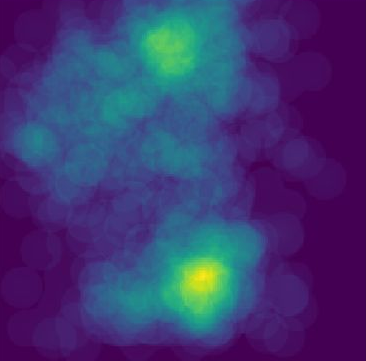
\includegraphics[width=0.30\linewidth]{./picsres/saliency_map_ori.png}& 
        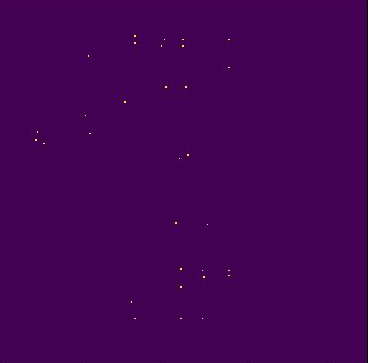
\includegraphics[width=0.30\linewidth]{./picsres/fixations_ori.png}& 
       
    
        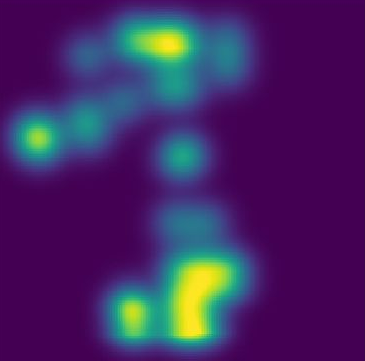
\includegraphics[width=0.30\linewidth]{./picsres/gaussians_ori.png}\\
       
         {\small Saliency Map} & {\small Fixations} & {\small Gaussian convoluted on fixations} \\
    \end{tabular}
    
    
    \caption{}
    \label{fig:fixat}
\end{figure}


\section{Implementation}

The deep learning part of the work have been implemented using the Python framework : Pytorch \cite{pytorch}. This framework offer a tensor based computation system with strong GPU acceleration. It also has a Deep Neural network building system, making the computations for the forward pass completely transparent and user made. This Framework is fast and powerful, completely suited for the work of designing a neural network and training it as we wanted.\\

All the prepossessing of data and its creation were made using python language and Numpy arrays. Same thing goes for the implementation of metrics and various code for loading data and organize training and testing. We didn't want to depend from too much libraries and limited their number to the strict minimum coding every algorithm ourselves in Python.\\

The computer we used for training and testing our network had a Nvidia 1080 as GPU, an Intel 40x Xeon E5-2630 and 132 GB of Ram available.

\subsection{Managing data in memory}
Memory space was not really a problem for us with the available space on the machine we use for training purposes. At least it was the case until we created our new dataset. With our augmented first dataset, we chose a simple but efficient way of loading the data directly in the 12GB V-RAM of our GPU. Doing so, for a small loading time we removed the transfer time between RAM and GPU, and increased the computing time during the training.
On the other hand we chose not to follow this strategy when training with our new dataset. As it is significantly bigger than the previous one it was impossible to load it all at one in the GPU memory. We chose to use the Pytorch's multi-workers functionality to ease and optimize the way our data was loaded in the GPU memory. This functionality creates threads in charge of loading batches into memory as they are needed by the training process.




\chapter{Results}

\section{Learning on training data}

The first important thing to assess when working with neural networks is how they learn. Firstly do the model is really learning anything and improving the quality of its knowledge. This is first assessed in section \ref{section:isitlearning}. We also need to check the efficiency of pretraining our network on the CAT2000 dataset  \cite{DBLP:journals/corr/BorjiI15}. We do it in section \ref{section:pretrain} and section \ref{section:strategies}, comparing two learning processes and strategies. Finally we will see the importance of data-augmentation in section \ref{section:augmentation}.

\subsection{Is the network learning? (bad title to be changed)}\label{section:isitlearning}
\begin{figure}[ht!]
\centering
    \begin{tabular}{c@{\hspace{0.1cm}}c@{\hspace{0.3cm}}c@{\hspace{0.1cm}}c}
        
\includegraphics[width=0.22\linewidth]{./picsres/weights_14_1.png} &
        
\includegraphics[width=0.22\linewidth]{./picsres/weights_14_2.png} &
        
\includegraphics[width=0.215\linewidth]{./picsres/weights_14_vgg_2_1.png}&
         
\includegraphics[width=0.222\linewidth]{./picsres/weights_14_vgg_2_2.png}
    \end{tabular}
\centering
    \begin{tabular}{c@{\hspace{4.5cm}}c}
       {\small 14th conv layer  } & {\small VGG16  14th conv layer } 
     \end{tabular}
     \begin{tabular}{c@{\hspace{0.1cm}}c@{\hspace{0.3cm}}c@{\hspace{0.1cm}}c}
        
\includegraphics[width=0.22\linewidth]{./picsres/weights_19_2_1.png} &
        
\includegraphics[width=0.22\linewidth]{./picsres/weights_19_2_2.png} &
        
\includegraphics[width=0.215\linewidth]{./picsres/weights_19_vgg_2_1.png}&
         
\includegraphics[width=0.222\linewidth]{./picsres/weights_19_vgg_2_2.png}
    \end{tabular}
     \begin{tabular}{c@{\hspace{5.5cm}}c}
              {\small 19th conv layer  } & {\small VGG16  19th conv layer }  

     \end{tabular}
    
    \caption{Comparison between the weights of our encoding network and VGG16}
    \label{fig:weights}
\end{figure}

When training a neural network, multiple ways can be used to see if the network is learning something and how does it learn it. The basic way would be to watch the loss progression and check if it is decreasing during the training. We can also check that the weights are not becoming random.
Figure \ref{fig:weights}, shows different filter/weights at various convolution layers. Their equivalent in the pretrained VGG are also displayed next to them. Those representation were produced by applying the forward pass of our network on a image with random values. By stopping at the desired layer and back-propagating from it while optimizing the image loss. The patterns formed are roughly the shape for which the learned filter is sensible.
We can see that our network has indeed learn something from our data as the weight have changed between our convolution layers and those of VGG. In particular for the 19th layer where we can see quite some difference between the two set of weights.

\subsection{Loss evolution}

\subsubsection{Loss evolution using pre-trained or not network}\label{section:pretrain}
We show in this section how pretraining our network on the visual attention dataset CAT2000 \cite{DBLP:journals/corr/BorjiI15} effect the overall training and our results. Figure \ref{fig:pretraining} show the effect of pretraining the network. We can see that without pretraining it the network is indeed learning but very slowly.
\begin{figure}[ht!]
    \centering
    \begin{tabular}{@{}c@{\hspace{0.1cm}}c@{\hspace{0.1cm}}c@{}}
        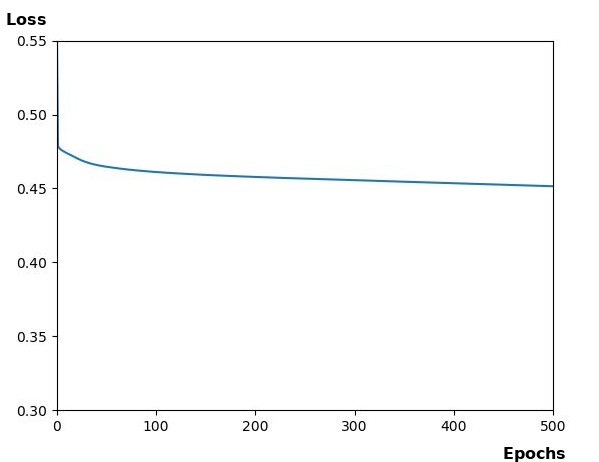
\includegraphics[width=0.518\linewidth]{./results/from_scratch_loss.png}& 
        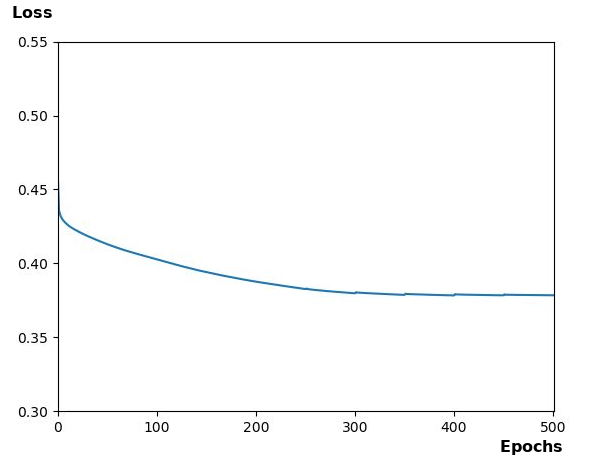
\includegraphics[width=0.505\linewidth]{./results/pretrained_loss.png}\\
        {\small Not pretrained network loss evolution} & {\small Pretrained network loss evolution} \\
       
    \end{tabular}
    \caption{Evolution of Loss for two networks, over 500 epochs. The first hasn't been pretrained while the second one has been pretrained on CAT2000 dataset \cite{DBLP:journals/corr/BorjiI15}}
    \label{fig:pretraining}
\end{figure}
Pretraining the network is effectively making the training process faster and improve results obtained. The explanation is coming from the decoder part of our network. Because we randomly initialized it it needs a lot of training to learn how to transform features extracted from the board to transform them into salient values. 
Training on the CAT2000 dataset becomes interested because of two main reasons : 
\begin{itemize}
    \item The features characterizing the CAT200 dataset are mainly the same as in the Imagenet dataset (faces,animals,plants etc..). And because our encoder part of the network is based in the imagenet pretrained VGG16, it doesn't need too much complementary training and can focus on training the decoder part. 
    \item The CAT2000 dataset offers a large amount of saliency map data. This allows our decoder part of the network to have enough resources to learn weights relevant for saliency map generation. 
\end{itemize}


\subsubsection{Effect of cyclical learning rate compared to standard decreasing learning rate}\label{section:strategies}

Figure \ref{fig:cyclicalr} shows the evolution of the loss during two training processes. The first one is an attempt using cyclical learning rate \cite{DBLP:journals/corr/Smith15a} and the second one decreasing the learning rate progressively. We can see that in the end, Cyclical learning rate  doesn't really affect the learning process in our case as we reach the same loss. 
\begin{figure}[ht!]
    \centering
    \begin{tabular}{@{}c@{\hspace{0.1cm}}c@{\hspace{0.1cm}}c@{}}
        \includegraphics[width=0.50\linewidth]{./pics/cyclical_loss.png}& 
        \includegraphics[width=0.50\linewidth]{./results/decreasing_lr.png}\\
        {\small  Using cyclical learning rate } & {\small Normal decreasing learning rate strategy} \\
       
    \end{tabular}
    \caption{Comparing two learning rate scheduling strategies}
    \label{fig:cyclicalr}
\end{figure}


However decreasing the learning rate is effectively reducing the loss faster than keeping the same learning rate for larger amounts of epochs. But after trying different learning rates and decreasing them or not, we end up finding that keeping a learning rate of 0.01 and training longer was an optimal strategy.

\subsection{Training our model on our dataset}
\begin{figure}[ht!]
    \centering
    \begin{tabular}{@{}c@{\hspace{0.1cm}}c@{}}
        \includegraphics[width=0.22\linewidth]{./results/configIX.png}& 
        \includegraphics[width=0.225\linewidth]{./results/newonly_IX_res.png}\\
        
        {\small  Configuration reference} & {\small Predicted saliency} \\
    \end{tabular}
    \caption{Example of how a network only trained on our dataset performs}
    \label{fig:newonly}
\end{figure}
The idea behind this dataset wasn't to use it as our main source of training data, but rather to use it to pretrain our network and lead the network to learn pieces and moves. Hypothetically with enough training and diversified data, it would be possible for the network to learn what to play or the different possibilities for a lot of configurations. Because of the dataset size, we had to reduce the training time to few hundred of epochs instead of thousands. When we stopped the training, the loss was still slowly decreasing, but as figure \ref{fig:newonly} shows, we still have a bias related to the number of opening being too important as explained in \ref{section:descpnewdataset0}.



\subsection{Data augmentation results}\label{section:augmentation}
An other interesting thing to test was the usefulness of the data augmentation. For that we trained two models with no data augmentation other than cutting the board into four parts. The first one was pretrained on CAT2000 dataset\cite{DBLP:journals/corr/BorjiI15} and the second one on the dataset we created. Both were trained during 2000 epochs with a learning rate of 0.01. The results for those training on the test data are presented in figure \ref{fig:augment} with a model trained using data augmentation and pretrained on our dataset. The metrics used in figure \ref{fig:augment} are explained in section \ref{seq:metrics}.
\begin{figure}[ht!]
    \centering
\begin{tabular}{|c|c|c|c|c|c|}
  \hline
  Model/Metrics & LCC & SIM & NSS & AUC-Judd & AUC-Borji \\
  \hline
  V1.0 & 0.46 & 0.59 & 0.25 & 0.44 & 0.59 \\
  V2.0 & 0.67 & 0.69 & 0.24 & 0.63 & 0.73 \\
  V3.0 & 0.529 & 0.604 & 0.207 & 0.739 & 0.792\\
  \hline
\end{tabular}
 \caption{Models : \textbf{V1.0} No data augmentation pretrained on our dataset  \textbf{V2.0}
 No data augmentation pretrained on CAT2000 \textbf{V3.0} pretained on new data and then trained normally}
 \label{fig:augment}
\end{figure}

\begin{figure}[ht!]
    \centering
    \begin{tabular}{@{}c@{\hspace{0.1cm}}c@{\hspace{0.1cm}}}
        {\small Configuration 1} & {\small Configuration 2}&
        \includegraphics[width=0.22\linewidth]{./picsres/XVII.png}& 
        \includegraphics[width=0.22\linewidth]{./picsres/XXIX.png}\\
         \includegraphics[width=0.22\linewidth]{./picsres/groundtruth_XVII.png}& 
        \includegraphics[width=0.22\linewidth]{./picsres/groundtruth_XXIX.png}\\
        
        \includegraphics[width=0.22\linewidth]{./picsres/noaugment_old_XVII.png}& 
        \includegraphics[width=0.22\linewidth]{./picsres/noaugment_old_XXIX.png}\\
         \includegraphics[width=0.22\linewidth]{./picsres/noaugment_new_XVII.png}& 
        \includegraphics[width=0.22\linewidth]{./picsres/noaugment_new_XXIX.png}\\

    \end{tabular}
    \caption{The first line shows the configuration, the second line their saliency map groundtruth, the third line is the result obtained with \textbf{V2.0}, the fourth line are the results obtained using \textbf{V1.0} }
    \label{fig:augmentres}
\end{figure}
From figure \ref{fig:augment} we can see few things straight away. First when we do not use any data augmentation , pretraining the network on CAT2000 (\textbf{V1.0)}, improves the performances compare to the model pretrained on our dataset (\textbf{V3.0}). Metrics such as linear correlation, similarity and normalized scan path, reveal a stronger correlation between our results and the ground truth for the pretrained on CAT2000 network. Concerning results for the AUC metrics, the difference is even more important as for the V2.0 model, its AUC results  can be classified as nearly fair while V1.0 is closer to failure. V3.0 model shows better performances than the same model without data augmentation (V1.0), but is not as good than V2.0 for LCC, SIM and NSS. On the other hand V3.0 is behaving better for AUC metrics with fair/nearly good results.



Using these metrics is not an easy way to visualize how the model performs on real examples. For that we show in Figure \ref{fig:augmentres}, the output of our network for two test data. The first row represent the chess configuration and the ground truth superposed on it. The second are the results obtained with our two networks. We can see several differences betwee the two training strategies and the groundtruth. For the configuration XVII, the network trained on CAT2000, correctly focus on both kings, rooks and the bishop as the groundtruth does. On the other hand the other network doesn't show as much interest for the rook and bishop on the right side of the board. Concerning the XXIX configuration, both networks takes the black king out but correctly "see" the white king and rook and the white queen too. The black queen and rook which are the key to the check mate are salient for both networks. 

\section{Evaluation data}

\subsection{Comparing results for differently trained networks}
\begin{figure}[ht!]
    \centering
    \begin{tabular}{@{}c@{\hspace{0.1cm}}c@{\hspace{0.1cm}}}
            {\small Configuration 1 } & {\small Configuration 2}\\
        \includegraphics[width=0.28\linewidth]{./picsres/XVII.png}& 
        \includegraphics[width=0.28\linewidth]{./picsres/XXIX.png}\\
         \includegraphics[width=0.28\linewidth]{./picsres/groundtruth_XVII.png}& 
        \includegraphics[width=0.28\linewidth]{./picsres/groundtruth_XXIX.png}\\
        \includegraphics[width=0.28\linewidth]{./picsres/final_old_network_XVII.png}& 
        \includegraphics[width=0.28\linewidth]{./picsres/final_old_network_XXIX.png}\\
         \includegraphics[width=0.28\linewidth]{./picsres/Final_new_XVII.png}& 
        \includegraphics[width=0.28\linewidth]{./picsres/Final_new_XXIX.png}\\
        
    \end{tabular}
    \caption{Comparison of prediction for two differently trained models on the two testing configuration. The \textbf{first row} is our configuration. The \textbf{second row} the groundtruth from the users eye tracking data. The \textbf{third row} are the prediction from the network pretrained on CAT2000 dataset (\textbf{V1.0}) and \textbf{the last row} from the network pretrained on our dataset (\textbf{V3.0})}
    \label{fig:modelcomp}
\end{figure}

\begin{figure}[ht!]
    \centering
\begin{tabular}{|c|c|c|c|c|c|}
  \hline
  Model & LCC & SIM & NSS & AUC-Judd & AUC-Borji \\
  \hline
  V1.0 & 0.568 & 0.621 & 0.318 & 0.640 & 0.725 \\
  V2.0 & 0.316 & 0.490 & 0.094 & 0.573 & 0.673 \\
  V3.0 & 0.529 & 0.604 & 0.207 & 0.739 & 0.792\\
  \hline
\end{tabular}
 \caption{Models : \textbf{V1.0} pretrained and normally trained,\textbf{V2.0} trained only on new data, \textbf{V3.0} pretained on new data and then trained normally}
 \label{table:modelcomp}
\end{figure}

To evaluate our work we need to compare few models trained differently. Figure \ref{table:modelcomp}, shows how well three of our models perform.
The first one (V1.0) has been pretrained on CAT200 and trained normally on our augmented dataset. The second one (V2.0) has only been trained on our dataset. And finally the third (V3.0) one has been pretrained on our dataset and then trained normally on our augmented dataset. Concerning correlation metrics (LCC,SIM,NSS), the model pretrained on CAT2000 is performing better than the others. But for the AUC metrics, the model pretrained on our dataset, is the one showing better results.\\



Figure \ref{fig:modelcomp} is about comparing the output of V1.0 and V3.0 for configurations XVII and XXIX. Concerning the latter, the area of fixation of V3.0 is larger and more spread than V1.0, but doesn't include the white rook and not completely the black king. V3.0 is also considering more of the board for XVII than V1.0, and even too much, but excluding the white bishop. We can see that it "fixates" the bottom right part of the board while there is nothing here. It could come from that for our dataset there are a lot of castling happening on this side of the board. This pattern could have been learned by the network.


\subsection{Comparing performances for different training/validation cut}

In this section we are going to compare, how choosing differently the testing and training data among our augmented dataset affects the performances (for the same amount of training epochs and same learning rate of 0.01). Figure \ref{table:comptraintest} showcases these differences. We can see that the model \textbf{V3.*} is on average better concerning AUC metrics where it can be considered as fair, while \textbf{V1.*} is better for correlation metrics.

\begin{figure}[ht!]
    \centering
\begin{tabular}{|c|c|c|c|c|c|}
  \hline
  Model & LCC & SIM & NSS & AUC-Judd & AUC-Borji \\
  \hline
  V1.0 & 0.568 & 0.621 & 0.318 & 0.640 & 0.725 \\
  V3.0 & 0.529 & 0.604 & 0.207 & 0.739 & 0.792\\
  V1.1 & 0.549 & 0.619 & 0.331 & 0.719 & 0.770 \\
  V3.1 & 0.372 & 0.553 & 0.210 & 0.618 & 0.705 \\
  V1.2 & 0.807 & 0.722 & 0.295 & 0.554 & 0.659 \\
  V3.2 & 0.804 & 0.750 & 0.277 & 0.703 & 0.758 \\
  \hline
\end{tabular}
 \caption{Comparison between models trained on differently cut training/testing set. \textbf{V1.*} is pretrained on CAT2000 and \textbf{V3.*} on our dataset. \textbf{V*.0} is using the two last configurations as testing data. \textbf{V*.1} is using the two first configurations as testing data. And 
 \textbf{V*.2} is using the two third and fourth configurations as testing data.} 
 \label{table:comptraintest}
\end{figure}





\subsection{Prediction examples and analysis }\label{section:examples}
In this section we will see how our networks performed on various configurations.
To create those configuration we used the board editor from Liches \footnote{\url{https://en.lichess.org/editor}}
The first one \ref{fig:empty} is the simplest possible. An empty board, which in theory would return none or random short fixations on the board. We can see that this is the case for V3.0 where there are nearly no visual attention except on the top left corner, and very short and limited one all over the board (lighter purple). For V1.0, there are a lot more fixations in the bottom left corner and all over the top and right top corner.  
\begin{figure}[ht!]
    \centering
    \begin{tabular}{@{}c@{\hspace{0.1cm}}c@{\hspace{0.1cm}}c@{}}
        \includegraphics[width=0.3\linewidth]{./results/empty.png}& 
        \includegraphics[width=0.3\linewidth]{./results/res_empty.png}&
        \includegraphics[width=0.3\linewidth]{./res2/empty_res_p.png}\\
        {\small An empty board  } & {\small V3.0 saliency map} &  {\small V1.0 saliency map}\\
       
    \end{tabular}
    \caption{The simplest configuration, and empty board}
    \label{fig:empty}
\end{figure}

The figure \ref{fig:queenking} depicts an other simple configuration. Here the black king is put in check by the white queen. We would expect fixations on the two pieces and on the vertical line between them showing their relation. V3.0 is close to  what we could expect but with some salient areas on the left part of the board. V1.0 on the other hand shows less saliency between the two pieces but some on the right part of the board.
\begin{figure}[ht!]
    \centering
    \begin{tabular}{@{}c@{\hspace{0.1cm}}c@{\hspace{0.1cm}}c@{}}
        \includegraphics[width=0.3\linewidth]{./results/queen_and_king.png}& 
        \includegraphics[width=0.3\linewidth]{./results/res2_sup.png}&
        \includegraphics[width=0.3\linewidth]{./results/queen_and_king_res_p_sup.png}\\
        {\small An simple configuration  } & {\small V3.0 saliency map} &  {\small V1.0 saliency map}
    \end{tabular}
    \caption{An other simple configuration with only one king and its opponent queen}
    \label{fig:queenking}
\end{figure}

Now we try a more complicated configurations. Figure \ref{fig:withqueen}, is showing the white king in check. The only possibility is to move the king. The expected salient areas would be the white rooks, white king and  white queen and the black knight if we consider the king in check.
\begin{figure}[ht!]
    \centering
    \begin{tabular}{@{}c@{\hspace{0.1cm}}c@{\hspace{0.1cm}}c@{}}
        \includegraphics[width=0.3\linewidth]{./results/check_config1.png}& 
        \includegraphics[width=0.3\linewidth]{./results/res_config1_sup.png}& \includegraphics[width=0.3\linewidth]{./results/config1_res_sup.png}\\
        {\small An simple configuration  } & {\small V3.0 saliency map} &  {\small V1.0 saliency map}
       
    \end{tabular}
    \caption{A bit more complicated configuration. The white king is in check}
    \label{fig:withqueen}
\end{figure}
 If we don't know the check rule, the white queen diagonal and rooks vertical lines would be salient as they can attack the enemy king this way.
Here V3.0 considers all pieces and the position from where the queen would put the enemy king in check. But rooks verticals are not considered. V1.0 is considering moving the right rook upward and put the king in check more salient with the black knight.\\




\begin{figure}[ht!]
    \centering
    \begin{tabular}{@{}c@{\hspace{0.1cm}}c@{\hspace{0.1cm}}c@{}}
        \includegraphics[width=0.3\linewidth]{./results/without_queen.png}& 
        \includegraphics[width=0.3\linewidth]{./results/without_queen_res_new_sup.png}& \includegraphics[width=0.3\linewidth]{./results/without_queen_res_old_sup.png}\\
        {\small An simple configuration  } & {\small V3.0 saliency map} &  {\small V1.0 saliency map}
       
    \end{tabular}
    \caption{Same configuration as in \ref{fig:withqueen} but without the queen}
    \label{fig:withoutqueen}
\end{figure}

Now we can try to remove the queen from previous configuration \ref{fig:withqueen}, which gives us the configuration \ref{fig:withoutqueen}.

We should expect the saliency to be the same as previously , but without the queen area and its diagonal, with a stronger saliency between the white king an the black knight. V3.0 is verifying part of those expectation, as the link between knight and king is stronger but strangely some salient area in front of the left rook appears stronger than previously. V1.0 on the other hand has reduced the overall saliency except for the enemy king.

\begin{figure}[ht!]
    \centering
    \begin{tabular}{@{}c@{\hspace{0.1cm}}c@{\hspace{0.1cm}}c@{}}
        \includegraphics[width=0.3\linewidth]{./results/only_pawns.png}& 
        \includegraphics[width=0.3\linewidth]{./results/pawns-res_sup.png}& \includegraphics[width=0.3\linewidth]{./results/pawns-res_p_sup.png}\\
        {\small An simple configuration  } & {\small V3.0 saliency map} &  {\small V1.0 saliency map}
       
    \end{tabular}
    \caption{A configuration with only 3 pawns}
    \label{fig:pawns}
\end{figure}
The configuration presented in \ref{fig:pawns} is quite simple as there are only three pawns. We expect to have the three pawns salient, but with a small saliency as they don't really have any purpose. Here V3.0 is corresponding to our expectation even adding the area in front of our right black pawn as it is a recurrently played piece. V1.0 however considers the cells in front of the right pawn but also some area on the right behind it and on the top right corner.

\begin{figure}[ht!]
    \centering
    \begin{tabular}{@{}c@{\hspace{0.1cm}}c@{\hspace{0.1cm}}c@{}}
        \includegraphics[width=0.30\linewidth]{./res2/opening.png}& 
        \includegraphics[width=0.30\linewidth]{./res2/pretrained_new_opening_res_sup.png} &
        \includegraphics[width=0.30\linewidth]{./res2/pretrained_old_opening_res_sup.png}\\
        {\small An simple configuration  } & {\small V3.0 saliency map} &  {\small V1.0 saliency map}
       
    \end{tabular}
    \caption{An opening with a bishop in danger}
    \label{fig:opening}
\end{figure}
Figure \ref{fig:opening} is different from the others, considering the number of pieces. Here the white bishop in B5 is in danger because of the black pawn in C6. The logic way to do is to move the bishop either back or on the left. V3.0  shows the area surrounding the king/queen of the enemy and including the white bishop (the king was in check the round before). V1.0 consider the bottom right region (castling area) to be more salient than the rest and doesn't include the white bishop.

\begin{figure}[ht!]
    \centering
    \begin{tabular}{@{}c@{\hspace{0.1cm}}c@{\hspace{0.1cm}}c@{}}
        \includegraphics[width=0.30\linewidth]{./res2/opening_black_side.png}& 
        \includegraphics[width=0.30\linewidth]{./res2/opening_black_side_new_sup.png} &
        \includegraphics[width=0.30\linewidth]{./res2/opening_black_side_old_sup.png}\\
        {\small An simple configuration  } & {\small V3.0 saliency map} &  {\small V1.0 saliency map}
       
    \end{tabular}
    \caption{Same opening as \ref{fig:opening}, but one round before, on the black side}
    \label{fig:opening_black_side}
\end{figure}
Reverting the figure \ref{fig:opening} to see the game from the black perspective one round before, gives us figure \ref{fig:opening_black_side}. Here V3.0 doesn't seem to taking in consideration the bishop putting the king in check, but is showing the black bishop on white cells which can be put in B5 to put the queen in danger. V1.0 consider most of the board with an accent on the surroundings of the black queen and white king, including the dangerous white bishop.


\begin{figure}[ht!]
    \centering
    \begin{tabular}{@{}c@{\hspace{0.1cm}}c@{\hspace{0.1cm}}c@{}}
        \includegraphics[width=0.30\linewidth]{./results/knight_and_pawns.png}& 
        \includegraphics[width=0.30\linewidth]{./results/knight_and_pawns_res_new_sup.png} &
        \includegraphics[width=0.30\linewidth]{./results/knight_and_pawns_res_old_sup.png}\\
        {\small An simple configuration  } & {\small V3.0 saliency map} &  {\small V1.0 saliency map}
       
    \end{tabular}
    \caption{A choice for a knight}
    \label{fig:choice}
\end{figure}
This last configuration (Figure \ref{fig:choice} ) shows a white knight having two choices. It can either kill the pawn and be killed by the queen or kill the queen and kill the pawn next round. We would expect the area around the three pieces to be salient as well as the space between them. V3.0 once more corresponds to our assumptions choosing the queen to be more salient with the knight. V1.0 chooses also the queen and the knight but add salient areas a bit everywhere on the board too. 
\chapter{Conclusion and Discussion}

From what we have seen in this report, training an auto-encoder network for the task of visual attention prediction is a difficult and very data dependent task. However we have shown that using data augmentation and task driven data, this task was possible. In this conclusion chapter we are going to review our results and assess them in relation to our starting hypothesis. Then we will discuss our work and what we have achieved and talk about where it could lead.
\section{Conclusion}
\subsection{Can we model Chess players visual attention?}

The answer to our research question is yes. Visual attention has already been a very proficient field of computer vision and Deep learning. For natural images several Deep models have shown great performances and suggest further improvement in the near future. Concerning visual attention for chess players our first attempt to model shows promising results. We showed that a network of the auto-encoder shape was able to learn to produce saliency map of the predicted attention of chess players. While we focus mainly on the Bottom-up approach for visual attention prediction, our model was able to extract features and patterns from limited data.


\subsection{Pretraining the network, improves its efficiency}

Concerning prior training of our model, we have proposed two main strategies. The first one is about using well known visual attention prediction dataset to train the decoder part into transforming features to salient or not regions. The second strategies is based on leading the way our network learn the pieces and moves. The first strategy manifested better performances and closer to the groundtruth results. However it was a bit struggling to generalize to new configurations we created, displaying some salient areas around the boundaries of the board.
However pretraining the decoder part of the network with such dataset seems to be a good idea as a way to initialize its weights.
\subsection{Is our top-down approach effective?}

Even if our top-down strategy of a new dataset leading the network to learn pieces and moves at the same time, proved to be working to produce saliency map when no visual attention prediction dataset is available. We will discuss how it could be improved in the discussion part of the report (Chapter \ref{chapter:discussion}), but we can assess some things about its performances:
\begin{itemize}
    \item The bias (more openings, so there are more salient areas on the player side) we announced in the method chapter, is verified as seen in figure \ref{fig:newonly}. However it is partially overthrown after training on the augmented dataset.
    \item The results from network pretrained on this dataset, are showing smaller salient areas focused on pieces. This is a direct consequence of how the dataset has been created, but is interesting as it correspond more to how beginner/intermediate players would look at the board.
    \item The network seems to be recognizing more pieces and their relation than pattern made by them. If we want to predict visual attention for beginner/intermediate players it is a good thing, but not for expert payers. However it shows that it is possible for a network to learn spatial relationship on top of pieces detection, just by using new data.
\end{itemize}

\subsection{Data augmentation}

As seen in section \ref{section:augmentation}, data augmentation is improving performances of our network when pretraining on our new dataset, but not really for other pretraining strategies. The amount of data added, is improving the locations of salient areas and what they are covering rather than the correspondence between the saliency map created and the groundtruth. We can definitely conclude that augmenting the data for our problem is useful especiall


\section{Discussion}
\subsection{How to improve our data}

Concerning the data we had to train our network, there several things we can say for its improvement :
\begin{itemize}
    \item Firstly its quantity. With only 11 configurations and around 30 users, it was clearly not enough for a Deep learning approach to be able to model and generalize our network results. The amount of users is sufficient but the number of configuration is not. One way to improve that would be to record eye tracking data for players playing full games for example during online tournaments  or even when casually training. With such data we could cover way more configurations and get more eye tracking data and from a larger panel of players expertise.
    \item Data should be big enough to create groups based on players skill. It has been shown in previous work that for board games such as chess, players depending on their expertise don't look at the game the same way. Doing this separation we could have 3 different networks all pretrained on the whole data, but finetuned on data from the 3 different players group : begginer, intermediates, experts. We would then have 3 different network able of modeling visual attention for their respective expertise group.
\end{itemize}

\subsection{New combination of top down and bottom up approach}
In this project we have seen that modeling visual attention for chess players is possible. This have been done mostly using a bottom up approach where the network base its prediction over graphical features. Patterns an configuration can be learned as they are extracted from the board's image itself. 
In the second part of the project we have worked on training our network on a more top-down approach where we highlight important pieces for each moves. 
An other way to learn visual attention based on the task is to learn how to execute the task. Here for chess the task is simple : win the game base on the rules of the game. A lot of work has been done on teaching chess expertise to computer from deep blue \cite{} to more recent work as AlphaZero \cite{}.
An idea to produce visual attention from chess expertise would be to use at each round the moves investigated by the network and highlight them. Doing so a map of salient pieces would appear.
With a bottom up and topdown maps we would need to find a way to combine them and learn from their combination. An weighted averaging between the too saliency map or a combination of loss would be techniques to investigate. With such two-ways network we could center salient area around moves to play and using at the same time the patterns learned from the board.\\

In the end we have open the investigation concerning visual attention prediction for chess players. This problem could also concern other board games such as GO, where the model used and its training would be the same, with just a variation of the data and game rules.




%\lipsum[2-4]
\chapter{Discussion}\label{chapter:discussion}



\appendix \chapter{Appendix} 


\section{Deep learning}\label{Annexe:deeplearning}
\subsection{Neural networks}
\subsubsection{A neuron}

Before talking about Convolutional neural network we could ask ourselves what are those neuron we are talking about. In biology the neuron can be represented as in the figure \ref{fig:bioneuron}. The information (input) enter the neuron coming from the dendrites, is processed by the neuron and continues its journey following the axon to the synapses where the connection to an other neuron or group of neurons is made.
\begin{figure}[h!]
   \centerline{\includegraphics[scale=0.30]{./pics/neuronb.png}}
   \caption{A representation of a biological Neuron}
   \label{fig:bioneuron}
\end{figure}

In machine learning, a neuron is roughly following the same idea. An input is taken processed using a function and an output is given to the next neuron or piece of software. This is represented in figure \ref{fig:artneuron}, several inputs are given to a neuron, with a bias. 

\begin{figure}[h!]
   \centerline{\includegraphics[scale=0.35]{./pics/ArtificialNeuron.png}}
   \caption{A representation of an artificial Neuron }
   \label{fig:artneuron}
\end{figure}

The output of equation \ref{eq:per} is given to an activation function here $f$ given in equation \ref{eq:relu}, which is a RELU function, most commonly used in Convulational neural network nowadays with the sigmoid function represented in equation \ref{eq:sig}. 

\begin{equation}
    y = \sum\limits_{i=1}^n w_ix_i  + bias
    \label{eq:per}
\end{equation}

\begin{equation}
    f(x) = 
 \begin{cases} 
      x & x >0 \\
      0 & otherwise
   \end{cases}
    \label{eq:relu}
\end{equation}

\begin{equation}
    f(x) = \frac{1}{1+ e^{-x}}
    \label{eq:sig}
\end{equation}


This is a basic neuron representation which is the one used in the perceptron algorithm \cite{Rosenblatt58theperceptron} which we are going to see later.

\subsubsection{The Perceptron or premises of modern machine learning}

In 1958 Rosenblatt introduced the perceptron, a probabilistic model modelling in a simpler way the way the brain process information. The goal was to define an algorithm where updatable weights are multiplied by the input to make a decision if the neuron is activated or not. For example for a binary classification problem it would tell us for sample to which class the belongs to, by learning a function separating classes.
The algorithm works as follow for all inputs :
\begin{enumerate}
    \item  Compute the output using the following equation: $x =w_ix_i + bias$ and $output = f(x) = 1 if x >0, -1$ otherwise
    \item Compute gradients : $\Delta w_i = \eta(target - output) x_i$ and $\Delta bias = \eta(target - output)$ ($\eta$ being the learning rate between 0 and 1)
    \item update weights : $w_i = w_i +\Delta w_i$ and $bias = bias + \Delta bias$
\end{enumerate}

In the end, by initializing weights at 0 we can learn a linear function separating our samples as in figure \ref{fig:class}.
\begin{figure}[ht!]
   \centerline{\includegraphics[scale=0.25]{./pics/linear.png}}
   \caption{A binary linear classification of some data}
   \label{fig:class}
\end{figure}

\subsubsection{Multi-layer perceptron/neural network}

A multi-layer perceptron looks as shown in figure \ref{fig:percp}. This is basically multiple neurons connected to each others as "layers". The activation can be a non linear one such as a Sigmoid or piece wise like RELU.
The forward pass (from input to output) is quite straight forward once we define the function $f$. But we also need to update our weights and here comes the idea of back propagation, which can be summed up as, how to learn from our mistakes. The algorithm for a multi-layer perceptron can be summed up as follow:
\begin{enumerate}
    \item Forward the input in the network using the equations we saw previously for each neuron.
    \item Compute the loss between the ouput and the target/ground truth.
    \item Backpropagate the loss in the network updating weights of each neuron.
\end{enumerate}

\begin{figure}[ht!]
   \centerline{\includegraphics[scale=2.0]{./pics/perceptron.jpeg}}
   \caption{A Multi-layer perceptron (source:cps0715.weebly.com)}
   \label{fig:percp}
\end{figure}

\subsubsection{Loss}

The loss can be obtain using several loss functions depending on the type of output, some famous one we can use are the following:

\textbf{The L1 loss}, which is the mean absolute value of the element-wise difference between input x and target y : $\ell(x, y) = mean(L), L = \{l_1,\dots,l_N\}^\top,  l_n = \left| x_n - y_n \right|$

\textbf{The mean squared error} :  $\ell(x, y) = mean(L), L = \{l_1,\dots,l_N\}^\top,  l_n = \left( x_n - y_n \right)^2 $

or the 


\textbf{Binary Cross Entropy loss } which is : $\ell(x, y) = mean(L) , L = \{l_1,\dots,l_N\}^\top, \\ l_n = \left[ y_n \cdot \log x_n + (1 - y_n) \cdot \log (1 - x_n) \right]$


\subsubsection{Backpropagation}

For the last part we need to execute the backpropagation algorithm. This algorithm can be summed up as , how much each weights impact the output and how to change it to reduce the Total error. Lets take the figure \ref{fig:artneuron} as an example and as an error function the square error $error = \sum\limits_{i=0}^n \frac{1}{2} (y_i - x_i)^2$ (the constant $\frac{1}{2}$ is here to cancel the exponent during differentiation). So applying forward pass we get an Error that we will call $E_{Total}$. Now for the backpropagation part we want to know how much $W_3$ change the $E_{Total}$, which can be written $\frac{ \delta E_{Total}}{\delta W_2}$, the partial derivative of $E_{Total}$ with respect to $W_2$ If we apply the chain rule considering figure \ref{fig:artneuron} we get equation \ref{eq:gradient}.

\begin{equation}
    \frac{ \delta E_{Total}}{\delta W_2} = \frac{ \delta E_{Total}}{\delta outputofneuron}  * \frac{ \delta outputofneuron}{\delta inputofneuron} * \frac{ \delta inputofneuron}{\delta W_2}
    \label{eq:gradient}
\end{equation}
We are going to simply the neuron a bit, by removing inputs to have only two inputs 1 and 2. We have $ E_{Total} = \frac{1}{2} (target - output)^2$ and $\frac{ \delta E_{Total}}{\delta outputofneuron} = 2 * \frac{1}{2} (target - output) * -1 + 0 = -(target - output)  $. Now if we consider that the output of the neuron is computer using sigmoid function \ref{eq:sig}, its partial derivative is $ output ( 1 - output)$. For the result of the neuron function that we call here $inputofneuron$, which is computed as  $ (x_1 * W_1) + (x_2 * W_2) + bias$, its partial derivative would be simply $ x_2$.\\

The calculations above can be summed up as $\frac{ \delta E_{Total}}{\delta W_2} = -(target- output) * output ( 1- output) * x_1 $ and taking $ \delta_2 = \frac{ \delta E_{Total}}{\delta outputofneuron}  * \frac{ \delta outputofneuron}{\delta inputofneuron}$ we get  $  \frac{ \delta E_{Total}}{\delta W_2} \delta_2 * x_2$, which is the usual notation for the "gradient" with respect to $W_2$.\\

Now we need to update the weight $W_2$, which is simply done as : $\textrm{new} W_2 = W_2 + \eta \delta W_2$, with $\eta$ our learning rate.\\

With hidden layers, it becomes a bit more difficult to update weights as they influence output hence error of following layers. This implies taking into consideration the effect of outputs neuron, and making the chain rule a bit more complex, but computation remain the same, and it is not really complicated to implement.
Appendix goes here...
%=========================================================


%=========================================================
\backmatter

\printbibliography
%\cleardoublepage % Goes to an odd page
%\pagestyle{empty} % no page number
%~\newpage % goes to a new even page

\end{document}